% Options for packages loaded elsewhere
\PassOptionsToPackage{unicode}{hyperref}
\PassOptionsToPackage{hyphens}{url}
%
\documentclass[
]{book}
\usepackage{amsmath,amssymb}
\usepackage{lmodern}
\usepackage{iftex}
\ifPDFTeX
  \usepackage[T1]{fontenc}
  \usepackage[utf8]{inputenc}
  \usepackage{textcomp} % provide euro and other symbols
\else % if luatex or xetex
  \usepackage{unicode-math}
  \defaultfontfeatures{Scale=MatchLowercase}
  \defaultfontfeatures[\rmfamily]{Ligatures=TeX,Scale=1}
\fi
% Use upquote if available, for straight quotes in verbatim environments
\IfFileExists{upquote.sty}{\usepackage{upquote}}{}
\IfFileExists{microtype.sty}{% use microtype if available
  \usepackage[]{microtype}
  \UseMicrotypeSet[protrusion]{basicmath} % disable protrusion for tt fonts
}{}
\makeatletter
\@ifundefined{KOMAClassName}{% if non-KOMA class
  \IfFileExists{parskip.sty}{%
    \usepackage{parskip}
  }{% else
    \setlength{\parindent}{0pt}
    \setlength{\parskip}{6pt plus 2pt minus 1pt}}
}{% if KOMA class
  \KOMAoptions{parskip=half}}
\makeatother
\usepackage{xcolor}
\IfFileExists{xurl.sty}{\usepackage{xurl}}{} % add URL line breaks if available
\IfFileExists{bookmark.sty}{\usepackage{bookmark}}{\usepackage{hyperref}}
\hypersetup{
  pdftitle={GUIA DE VICAL: Calculadora de indices de vegetación},
  pdfauthor={INIFAP: Sergio Jiménez-Jiménez; Mariana Marcial-Pablo; Waldo Ojeda-Bustamante; Ernesto Sifuentes-Ibarra; Marco Inzunza-Ibarra, Ignacio Sánchez-Cohen},
  pdflang={es-MX},
  hidelinks,
  pdfcreator={LaTeX via pandoc}}
\urlstyle{same} % disable monospaced font for URLs
\usepackage[margin=2cm]{geometry}
\usepackage{color}
\usepackage{fancyvrb}
\newcommand{\VerbBar}{|}
\newcommand{\VERB}{\Verb[commandchars=\\\{\}]}
\DefineVerbatimEnvironment{Highlighting}{Verbatim}{commandchars=\\\{\}}
% Add ',fontsize=\small' for more characters per line
\usepackage{framed}
\definecolor{shadecolor}{RGB}{248,248,248}
\newenvironment{Shaded}{\begin{snugshade}}{\end{snugshade}}
\newcommand{\AlertTok}[1]{\textcolor[rgb]{0.94,0.16,0.16}{#1}}
\newcommand{\AnnotationTok}[1]{\textcolor[rgb]{0.56,0.35,0.01}{\textbf{\textit{#1}}}}
\newcommand{\AttributeTok}[1]{\textcolor[rgb]{0.77,0.63,0.00}{#1}}
\newcommand{\BaseNTok}[1]{\textcolor[rgb]{0.00,0.00,0.81}{#1}}
\newcommand{\BuiltInTok}[1]{#1}
\newcommand{\CharTok}[1]{\textcolor[rgb]{0.31,0.60,0.02}{#1}}
\newcommand{\CommentTok}[1]{\textcolor[rgb]{0.56,0.35,0.01}{\textit{#1}}}
\newcommand{\CommentVarTok}[1]{\textcolor[rgb]{0.56,0.35,0.01}{\textbf{\textit{#1}}}}
\newcommand{\ConstantTok}[1]{\textcolor[rgb]{0.00,0.00,0.00}{#1}}
\newcommand{\ControlFlowTok}[1]{\textcolor[rgb]{0.13,0.29,0.53}{\textbf{#1}}}
\newcommand{\DataTypeTok}[1]{\textcolor[rgb]{0.13,0.29,0.53}{#1}}
\newcommand{\DecValTok}[1]{\textcolor[rgb]{0.00,0.00,0.81}{#1}}
\newcommand{\DocumentationTok}[1]{\textcolor[rgb]{0.56,0.35,0.01}{\textbf{\textit{#1}}}}
\newcommand{\ErrorTok}[1]{\textcolor[rgb]{0.64,0.00,0.00}{\textbf{#1}}}
\newcommand{\ExtensionTok}[1]{#1}
\newcommand{\FloatTok}[1]{\textcolor[rgb]{0.00,0.00,0.81}{#1}}
\newcommand{\FunctionTok}[1]{\textcolor[rgb]{0.00,0.00,0.00}{#1}}
\newcommand{\ImportTok}[1]{#1}
\newcommand{\InformationTok}[1]{\textcolor[rgb]{0.56,0.35,0.01}{\textbf{\textit{#1}}}}
\newcommand{\KeywordTok}[1]{\textcolor[rgb]{0.13,0.29,0.53}{\textbf{#1}}}
\newcommand{\NormalTok}[1]{#1}
\newcommand{\OperatorTok}[1]{\textcolor[rgb]{0.81,0.36,0.00}{\textbf{#1}}}
\newcommand{\OtherTok}[1]{\textcolor[rgb]{0.56,0.35,0.01}{#1}}
\newcommand{\PreprocessorTok}[1]{\textcolor[rgb]{0.56,0.35,0.01}{\textit{#1}}}
\newcommand{\RegionMarkerTok}[1]{#1}
\newcommand{\SpecialCharTok}[1]{\textcolor[rgb]{0.00,0.00,0.00}{#1}}
\newcommand{\SpecialStringTok}[1]{\textcolor[rgb]{0.31,0.60,0.02}{#1}}
\newcommand{\StringTok}[1]{\textcolor[rgb]{0.31,0.60,0.02}{#1}}
\newcommand{\VariableTok}[1]{\textcolor[rgb]{0.00,0.00,0.00}{#1}}
\newcommand{\VerbatimStringTok}[1]{\textcolor[rgb]{0.31,0.60,0.02}{#1}}
\newcommand{\WarningTok}[1]{\textcolor[rgb]{0.56,0.35,0.01}{\textbf{\textit{#1}}}}
\usepackage{longtable,booktabs,array}
\usepackage{calc} % for calculating minipage widths
% Correct order of tables after \paragraph or \subparagraph
\usepackage{etoolbox}
\makeatletter
\patchcmd\longtable{\par}{\if@noskipsec\mbox{}\fi\par}{}{}
\makeatother
% Allow footnotes in longtable head/foot
\IfFileExists{footnotehyper.sty}{\usepackage{footnotehyper}}{\usepackage{footnote}}
\makesavenoteenv{longtable}
\usepackage{graphicx}
\makeatletter
\def\maxwidth{\ifdim\Gin@nat@width>\linewidth\linewidth\else\Gin@nat@width\fi}
\def\maxheight{\ifdim\Gin@nat@height>\textheight\textheight\else\Gin@nat@height\fi}
\makeatother
% Scale images if necessary, so that they will not overflow the page
% margins by default, and it is still possible to overwrite the defaults
% using explicit options in \includegraphics[width, height, ...]{}
\setkeys{Gin}{width=\maxwidth,height=\maxheight,keepaspectratio}
% Set default figure placement to htbp
\makeatletter
\def\fps@figure{htbp}
\makeatother
\setlength{\emergencystretch}{3em} % prevent overfull lines
\providecommand{\tightlist}{%
  \setlength{\itemsep}{0pt}\setlength{\parskip}{0pt}}
\setcounter{secnumdepth}{5}
\ifLuaTeX
\usepackage[bidi=basic]{babel}
\else
\usepackage[bidi=default]{babel}
\fi
\babelprovide[main,import]{spanish}
% get rid of language-specific shorthands (see #6817):
\let\LanguageShortHands\languageshorthands
\def\languageshorthands#1{}
\usepackage{booktabs}
\usepackage{amsthm}
\makeatletter
\def\thm@space@setup{%
  \thm@preskip=8pt plus 2pt minus 4pt
  \thm@postskip=\thm@preskip
}
\makeatother
\usepackage{titling}
\pretitle{\begin{center} 
\includegraphics[width=2in,height=2in]{./images/1.png}\LARGE\\}
\posttitle{\end{center}}
\ifLuaTeX
  \usepackage{selnolig}  % disable illegal ligatures
\fi
\usepackage[]{natbib}
\bibliographystyle{apalike}

\title{GUIA DE VICAL: Calculadora de indices de vegetación}
\author{INIFAP: Sergio Jiménez-Jiménez; Mariana Marcial-Pablo; Waldo Ojeda-Bustamante; Ernesto Sifuentes-Ibarra; Marco Inzunza-Ibarra, Ignacio Sánchez-Cohen}
\date{2022-06-07}

\begin{document}
\maketitle

{
\setcounter{tocdepth}{1}
\tableofcontents
}
\hypertarget{bienvenidos}{%
\chapter*{Bienvenidos}\label{bienvenidos}}
\addcontentsline{toc}{chapter}{Bienvenidos}

\begin{center}
\includegraphics{./images/LogoVICAL} \end{center}

Este sitio es una \emph{guía} para usar la herramienta \textbf{VICAL} desarrollada dentro de Google Earth Engine (GEE). VICAL es util para calcular de manera \textbf{online} 23 índices de vegetación (empleados comúnmente en aplicaciones agrícolas) de cualquier poligono(s) del mundo (digitalizado por el usuario o archivo vector) usando imágenes LandSat y Sentinel-2. Esto se logra sin que el usuario descargue/cargue imágenes satelitales o escriba una solo línea de código, solo necesita tener una conexión a internet.

Puede accesar a \textbf{VICAL} desde la dirección
\url{https://inifapcenidraspa.users.earthengine.app/view/vical}

\begin{figure}

{\centering 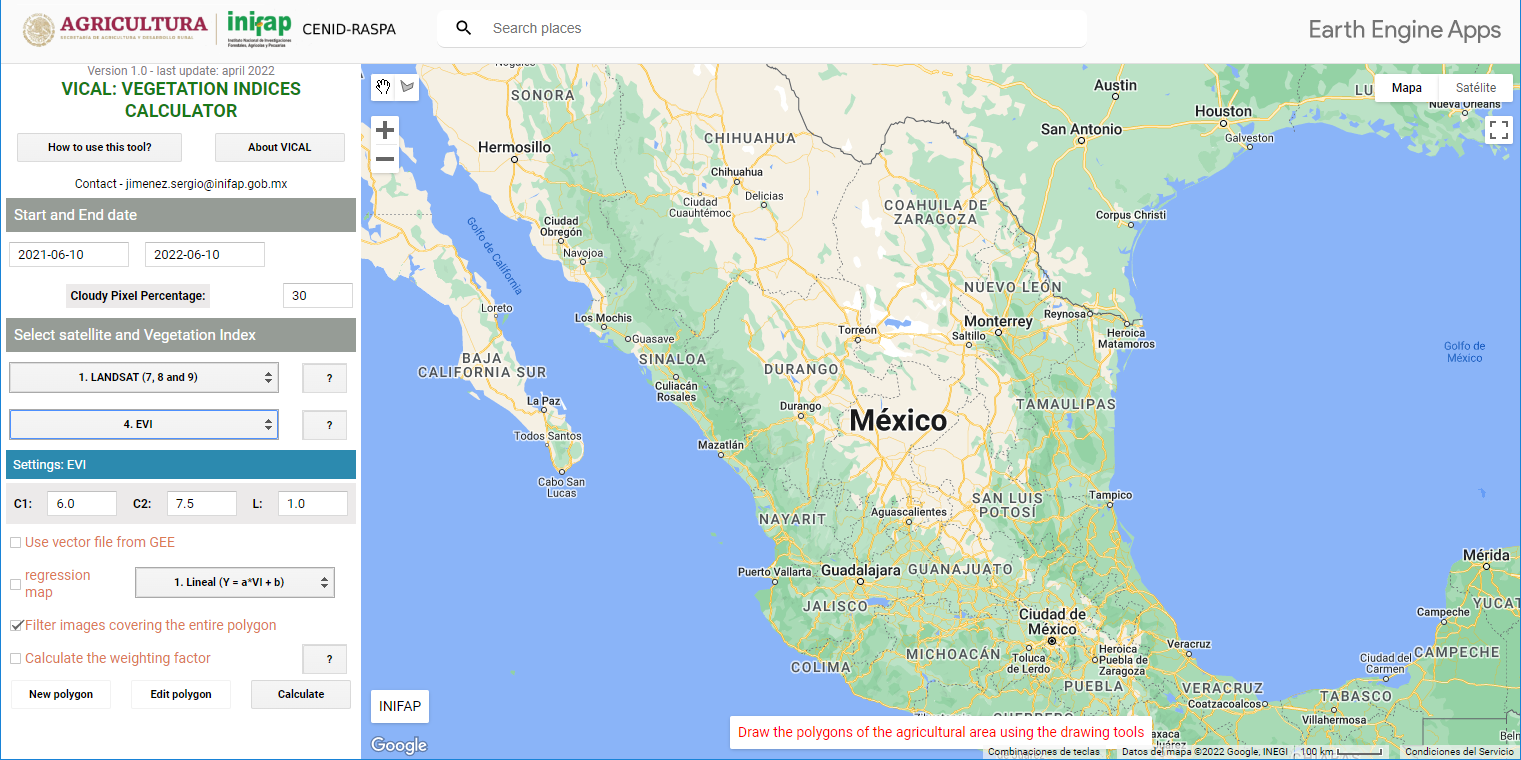
\includegraphics[width=0.9\linewidth]{./images/Figure4} 

}

\caption{Vista principal de VICAL}\label{fig:fig2}
\end{figure}

Este trabajo fue desarrollado por investigadores del \textbf{INIFAP CENID-RASPA} y \textbf{CEVAF}. Dentro de las mejoras que se planean en VICAL, es que mediante experimentación se logre la calibración de variables biofísicas de interés para diversos cultivos usando \emph{indices de vegetacion (IV)}; y estos resultados estén disponibles en \textbf{VICAL} para que sea útil a otras personas y asi puedan monitorear facilmente variables relacionadas con ingenieria de riego.

\emph{Vuelva a consultar de vez en cuando para conocer las nuevas aplicaciones de GEE, los scripts de ejemplo y las actualizaciones de VICAL. Puede intentar hacer una actualización completa en el sitio para asegurarse de ver los cambios recientes (lo que está viendo podría ser una versión del sitio previamente almacenada en caché)}

\emph{Sí tiene alguna duda o sugerencia o quiere participar en el proyecto puede escribir al correo \textbf{\href{mailto:jimenez.sergio@inifap.gob.mx}{\nolinkurl{jimenez.sergio@inifap.gob.mx}}}}

\hypertarget{intro}{%
\chapter{Introducción}\label{intro}}

El objetivo de esta sección es presentar los alcances de \textbf{VICAL} y como utilizarlo, ademas de, como implementar las librerías en cualquier Script de GEE. Se describen los índices de vegetación considerados en el programa y las colecciones de imagenes que se usan para calcularlo, cuáles son los resultados y cómo están formateados.


\includegraphics[width=0.25\linewidth]{./images/1}

VICAL fue desarrollado dentro de GEE \url{https://earthengine.google.com/} y fue codificado en JavaScript desde Earth Engine Code Editor \url{https://code.earthengine.google.com/}.

\hypertarget{alcances}{%
\section{Alcances}\label{alcances}}

Los principios de diseño para \textbf{VICAL} fueron que deberia proporcionar para cualquier área (definida por el usuario) donde exista una imagen Landsat o Sentinel-2 la estimación de diferentes IVs aplicados en agricultura, además, de graficar la serie de tiempo de dicho índice para esa zona en el rango de fecha establecido por el usuario. \textbf{Todo sin que el usuario escriba una sola linea de codigo dentro de GEE o que lleve a cabo el pre-procesamiento de las imágenes.}

VICAL tiene tres principales funciones:

\textbf{1.-} Mapas de índices de vegetación usando imágenes (libres de nubes) LandSat (4, 5, 7,8 y 9) y Sentinel-2 de cualquier poligono digitalizado por el usuario o archivo vector.

\textbf{2.-} El despliegue de series de tiempo de Indices de vegetación (media y desviación estándar) para polígonos (dibujados por el usuario o archivo vector) en un tiempo fijo con imagenes Landsat, sentinel o ambos.

\textbf{3.-} Mapa de regresiones usando los IVs o productividad relativa.

En esta herramientas, se puede configurar algunos coeficientes de IV como en EVI, SAVI, entre otros.

Creemos que la herramienta \textbf{VICAL} ahorra tiempo y evita el procedimiento trivial repetitivo asociado a los cálculos de IVs ``manuales'' (descarga de imágenes, procesamiento, etc.), que demanda diferentes tipos de software, que pueden conducir a errores humanos.

VICAL puede ser empleado para extraer rápidamente valores de índices de vegetación para su calibración en variables biofísicas agrícolas.

\hypertarget{Sat}{%
\chapter{Satélites- Colección de imagenes}\label{Sat}}

VICAL utiliza las colecciones de imágenes de reflectancia de la superficie terrestre corregidas atmosféricamente de LandSat (misiones 4, 5, 7, 8 y 9, con imágenes desde 1982 hasta el presente) y Sentinel-2.

En la Tabla \ref{tab:Sat} se muestra las características generales de estas colecciones de imágenes y el código de la colección de imágenes en GEE

\begin{table}

\caption{\label{tab:Sat}Colección de imagenes Landsat y Sentinel de GEE considerados en VICAL}
\centering
\begin{tabular}[t]{lll}
\toprule
Sensor & Dataset.availability & Collection.ID\\
\midrule
Landsat-4 TM & 22/08/1982 - 24/06/1993 & LANDSAT/LT04/C02/T1\_L2\\
Landsat-5 TM & 16/03/1993 – 05/05/2012 & LANDSAT/LT05/C02/T1\_L2\\
Landsat-7 ETM+ & 01/01/1999-present & LANDSAT/ LC08 /C01/T1\_L2\\
Landsat-8 OLI & 11/04/2013- present & LANDSAT/LE07/C01/T1\_L2\\
Landsat-9 OLI-2 & 31/10/2021- present & LANDSAT/LC09/C02/T1\_L2\\
\addlinespace
Sentinel-2 (MSI) & 28/03/2017-present & COPERNICUS/S2\_SR\_HARMONIZED\\
\bottomrule
\end{tabular}
\end{table}

La ubicación de las diferentes bandas espectrales de estos sensores se muestra en la Figura \ref{fig:figS1}.

\begin{figure}

{\centering 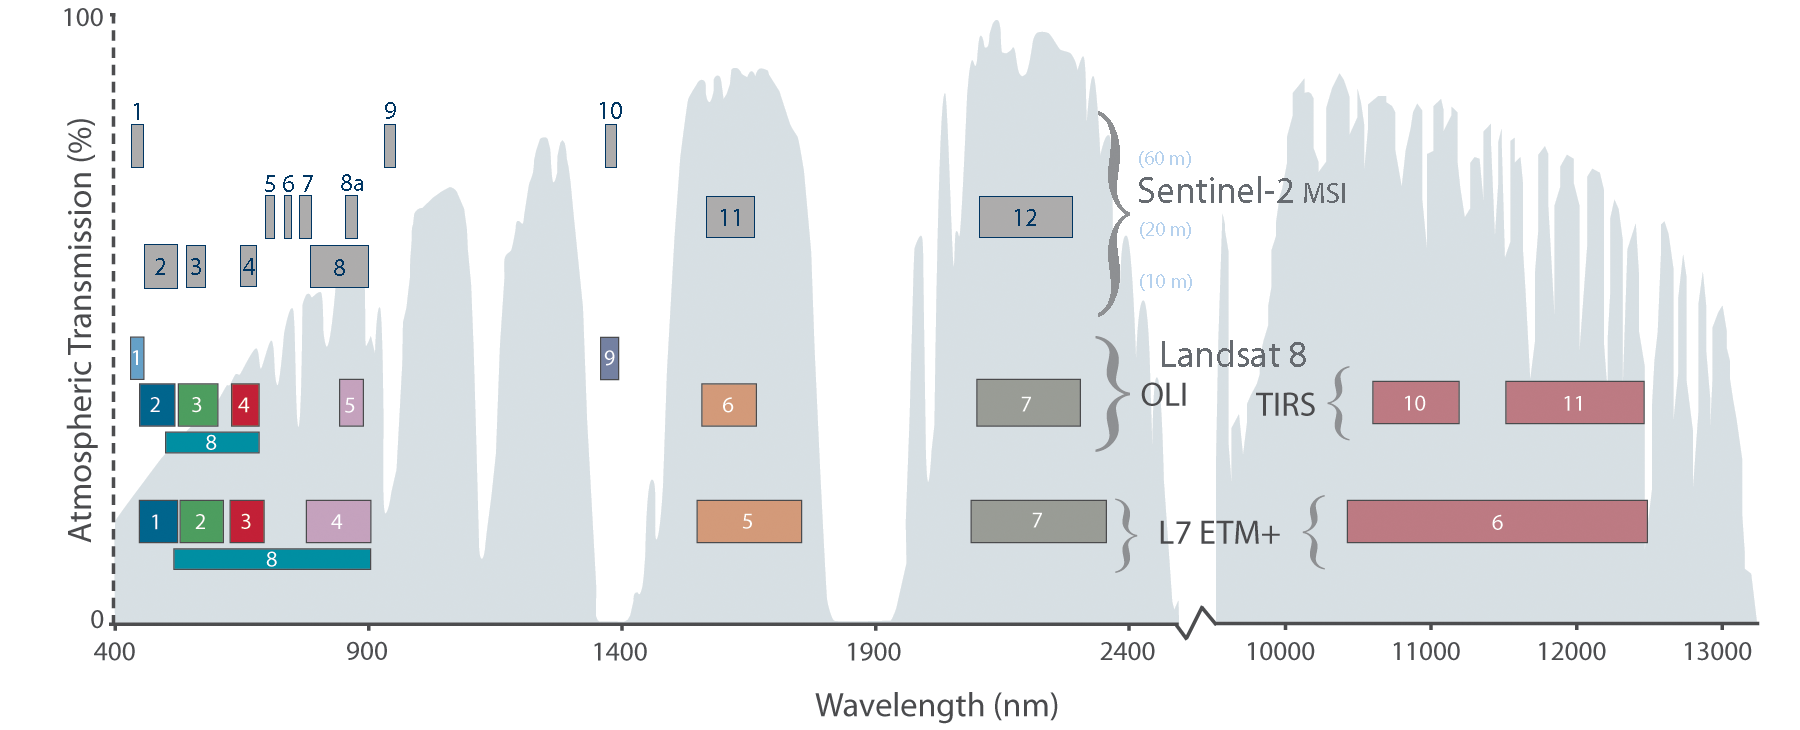
\includegraphics{./images/Figure21} 

}

\caption{Comparación de Lansat y Sentinel-2 y ubicacion de las bandas espectrales. Los números indican el número de bandas espectrales consideradas en cada sensor.}\label{fig:figS1}
\end{figure}

\hypertarget{Iveg}{%
\chapter{Indices de Vegetación}\label{Iveg}}

Los IVs permiten la relación cuantitativa y funcional con diferentes parámetros o variables de la vegetación. Son 23 IV considerados en VICAL y son los que comunmente se utilizan en aplicaciones agricolas \citep{Bannari2009},\citep{Xue2017}.

Los nombres de estos indices asi como su abreviatura se muestran en la siguiente lista:\\
\textbf{1: ARVI}: Atmospherically resistant vegetation index*
\[
ARVI = \frac{p(NIR-rb)}{NIR+rb};     
\]
\[
rb = {R-γ(B-R)}; \thinspace \thinspace  Valor \thinspace por \thinspace defecto: \thinspace γ=1.0 
\]

\textbf{2: ATSAVI}: Adjusted transformed soil-adjusted vegetation index\emph{
\[
ATSAVI = \frac{a(NIR-aR-b)}{(R+aNIR-ab+X(1+a^2))};
\]
\[
\thinspace \thinspace  Valor \thinspace por \thinspace defecto: \thinspace a= 1 ;\thinspace b=0; \thinspace X= 0.08      
\]
\textbf{3: DVI: } Difference vegetation index
\[
DVI = {(NIR-R)} ;   
\]
\textbf{4: EVI}}: Enhanced vegetation index
\[
EVI = \frac{2.5*(NIR-R)}{NIR+C_1 R-C_2 B+L};     
\]
\[
\thinspace \thinspace  Valor \thinspace por \thinspace defecto: \thinspace C_1= 6.0 ;\thinspace C_2=7.5; \thinspace L= 1.0      
\]
\textbf{5: EVI2}*: Enhanced vegetation index
\[
EVI2 = \frac{2.5*(NIR-R)}{NIR+C_1 R+1}; \thinspace \thinspace  Valor \thinspace por \thinspace defecto: \thinspace C_1= 2.4      
\]
\textbf{6: GNDVI}: Green normalized difference vegetation index
\[
GNDVI = \frac{NIR-G}{NIR+G};     
\]
\textbf{7: MSAVI2}: Modified soil adjusted vegetation index
\[
MSAVI2 = \frac{(2NIR+1)-\sqrt((2NIR+1)^2-8(NIR-R))}{2};     
\]
\textbf{8: MSI}: Moisture stress index
\[
MSI = \frac{SWIR_1}{NIR};     
\]
\textbf{9: MTVI}: Modified triangular vegetation index
\[
MTVI ={1.2[1.2*(NIR-G)-2.5*(R-G)]};     
\]

\textbf{10: MTVI2}: Modified triangular vegetation index-2
\[
MTVI2 = \frac{1.2[1.2*(NIR-G)-2.5*(R-G)]}{\sqrt((2NIR+1)^2-(6NIR-5\sqrt(R))-0.5)};     
\]
\textbf{11: NDTI}: Normalized difference tillage index (NDTI)
\[
NDTI = \frac{SWIR_1-SWIR_2}{SWIR_1+SWIR_2};     
\]
\textbf{12: NDVI}: Normalized difference vegetation index
\[
NDVI = \frac{NIR-R}{NIR+R};     
\]
\textbf{13: NDWI}: Normalized difference water index
\[
NDWI = \frac{NIR-SWIR_1}{NIR+SWIR_1};     
\]
\textbf{14: OSAVI}: Optimized soil adjusted vegetation index\emph{
\[
OSAVI = \frac{1.16*(NIR-R)}{NIR+R+X}; \thinspace \thinspace  Valor \thinspace por \thinspace defecto: \thinspace X= 0.16     
\]
\textbf{15: RDVI}: Renormalized difference vegetation index
\[
RDVI = \frac{NIR-R}{\sqrt(NIR+R)};     
\]
\textbf{16: RI}: Redness index
\[
RI = \frac{p(NIR-G)}{NIR+G};     
\]
\textbf{17: RVI}: Ratio vegetation index
\[
RVI = \frac{R}{NIR};     
\]
\textbf{18: SAVI}}: Soil adjusted vegetation index
\[
SAVI = \frac{(NIR-R)}{NIR+R+L} (1+ L);    \thinspace \thinspace  Valor \thinspace por \thinspace defecto: \thinspace L= 0.5  
\]
\textbf{19: TVI}: Triangular vegetation index
\[
TVI = 0.5*{[120(NIR-G)-200(R-G)]};     
\]
\textbf{20: TSAVI}\emph{: Transformed soil adjusted vegetation index
\[
TSAVI = \frac{a(NIR-aR-b)}{R+aNIR-ab};  \thinspace \thinspace  Valor \thinspace por \thinspace defecto: \thinspace a= 1,   \thinspace b=0.    
\]
\textbf{21: VARI}: Visible atmospherically resistant index
\[
VARI = \frac{G-R}{G+R-B};     
\]
\textbf{22: VIN}: Vegetation index number or simple ratio
\[
VIN = \frac{NIR}{R};     
\]
\textbf{23: WDRVI}}: Wide dynamic range vegetation index
\[
WDRVI = \frac{∝NIR-R}{∝NIR+R)}; \thinspace \thinspace  Valor \thinspace por \thinspace defecto: \thinspace ∝= 0.2   
\]

VICAL permite al usuario configurar algunos parámetros de VIs (como \textbf{ARVI, ATSAVI, EVI, EVI2, OSAVI, SAVI, ATSAVI y WDRVI}), es decir, todos aquellos IVs que necesitan, además de las bandas de espectro, alguna variable de ajuste

El nombre de las bandas con las abreviaturas que se emplearon en las ecuaciones de los IVs se muestra en la Tabla \ref{tab:inOMBRE}.

\begin{table}

\caption{\label{tab:inOMBRE}Abreviatura de las bandas espectrales empleadas en las ecuaciones de los IV}
\centering
\begin{tabular}[t]{ll}
\toprule
Abreviatura & Nombre\\
\midrule
B & Azul/Blue\\
G & Verde/Green\\
R & Rojo/Red\\
RE & Borde Rojo/Red edge\\
NIR & Infrarrojo Cercano /Near infrared\\
\addlinespace
SWIR1 & Infrarrojo de onda corta 1/Shortwave infrared 1\\
SWIR2 & Infrarrojo de onda corta 2/Shortwave infrared 2\\
\bottomrule
\end{tabular}
\end{table}

\emph{Si deseas agregar algun indice de vegetación puedes escribirnos al correo \href{mailto:jimenez.sergio@inifap.gob.mx}{\nolinkurl{jimenez.sergio@inifap.gob.mx}}}

\hypertarget{configuraciuxf3n}{%
\chapter{Configuración}\label{configuraciuxf3n}}

Antes de calcular los IVs en VICAL se deben seleccionar una serie de parámetros que corresponden a la configuración.

\hypertarget{configuraciuxf3n-general}{%
\section{Configuración General}\label{configuraciuxf3n-general}}

En principio, para estimar el IV de cualquier superficie el usuario tiene dos opciones: \emph{i) digitalizar polígonos o ii) Usar un archivo vector de GEE}. Además, es necesario configurar una serie de opciones, estos son:

\textbf{1). Rango de fechas: } Se debe ingresar una fecha inicial y final en que desea estimar estos índices de vegetación (Figura \ref{fig:figG1}). La fecha deben tener el siguiente formado: \emph{Cuatro dígitos para el año, dos para el mes y dos para el día (AAAA-MM-DD)}.

\begin{figure}

{\centering 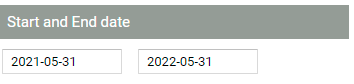
\includegraphics{./images/Figure1} 

}

\caption{TexBox de Rango de fechas}\label{fig:figG1}
\end{figure}

VICAL utiliza este intervalo de fechas para buscar imágenes disponibles y con estas estimar valores del índice de vegetación. VICAL por defecto establece la fecha final como la fecha actual y la fecha inicial un año atrás a la fecha actual.

\textbf{2) porcentaje de nubes: } Se debe ingresar un umbral máximo de nubes en las imágenes, por defecto es establecido en 30\% (Figura \ref{fig:figG2}).

\begin{figure}

{\centering 
\includegraphics{./images/Figure2} 

}

\caption{TexBox de umbral de porcentaje de nubes}\label{fig:figG2}
\end{figure}

\textbf{3). Satélite: } de los satélites LandSat y Sentinel-2 (descritos en la sección \ref{Sat} \textbf{Satélite}), se derivan cuatro opciones disponibles (Figura \ref{fig:figG3}):

\begin{figure}

{\centering 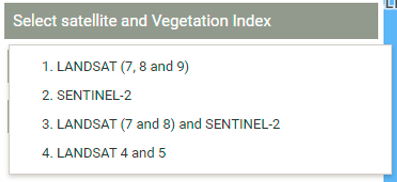
\includegraphics{./images/Figure3} 

}

\caption{Satelites y sensores disponibles en VICAL}\label{fig:figG3}
\end{figure}

~\emph{\textbf{i) Landsat (7, 8 y 9):} proporciona imágenes LandSat de los sensores 7, 8 y 9 que se encuentren dentro del intervalo definido y con un umbral máximo de nubes. Los datos de Landsat 7 ETM+ se ajustaron espectralmente a las bandas espectrales de Landsat 8 y 9 (OLI y OLI-2) usando el procedimiento recomendado por \citep{Roy2016}, para generar un solo conjunto de datos armonizados.}

~\emph{\textbf{ii) Sentinel-2:} solo proporciona imágenes Sentinel-2 que se encuentren dentro del intervalo definido y con el umbral máximo de nubes.}

~\emph{\textbf{iii) Landsat (7, 8 y 9) y Sentinel-2}: Proporciona tanto imágenes Landsat (7, 8 y 9) como Sentinel-2. Los datos MSI (Sentinel-2) se ajustan espectralmente a las bandas espectrales Landsat 8 y 9 (OLI y OLI-2) usando el procedimiento recomendado por \citep{Claverie2018}. Los datos de Landsat 7 ETM+ se ajustaron espectralmente a las bandas espectrales de Landsat 8 y 9 (OLI y OLI-2) usando el procedimiento recomendado por \citep{Roy2016}. De tal manera que se genera un solo conjunto de datos armonizados.}

~\emph{\textbf{iv) Landsat (4 y 5):} Proporciona imágenes LandSat de los sensores 4 y 5 que se encuentren dentro del intervalo definido y con un umbral máximo de nubes.}

\textbf{4). Índice de vegetación: } El usuario puede seleccionar entre 23 IVs comúnmente empleadas en aplicaciones agrícolas (Figura \ref{fig:figG4}), para revisar las fórmulas de cada índice de vegetación ver sección \ref{Iveg} \textbf{Índices de vegetación.}.

\begin{figure}

{\centering 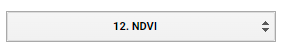
\includegraphics{./images/Figure5} 

}

\caption{Selector de Indices de vegetción}\label{fig:figG4}
\end{figure}

\begin{figure}

{\centering 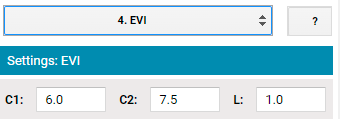
\includegraphics{./images/Figure5.1} 

}

\caption{Coeficientes de IV}\label{fig:figG5}
\end{figure}

\textbf{5) otras funciones adicionales: } VICAL permite seleccionar opciones adicionales (Figura \ref{fig:figG6}), por ejemplo:

\begin{figure}

{\centering 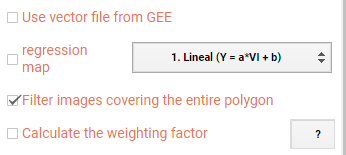
\includegraphics{./images/Figure9} 

}

\caption{Opciones en VICAL}\label{fig:figG6}
\end{figure}

\emph{\textbf{i) Usar un archivo vector de GEE:} Como se mencionó en la parte inicial de esta sección, el usuario puede usar un archivo vector de GEE (tipo polígono). Cuando se selecciona esta opción se debe ingresar una dirección URL del archivo vector que ha sido cargado a GEE (Figura \ref{fig:figG7}), de esta manera, aunque existan polígonos digitalizados VICAL reconoce que se deben calcular los índices de vegetación sobre los polígonos del archivo vector. }

\begin{figure}

{\centering 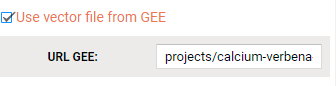
\includegraphics{./images/Figure10} 

}

\caption{URL archivo vector de GEE}\label{fig:figG7}
\end{figure}

\emph{\textbf{ii) Mapa de regresión:} El usuario puede obtener como resultado un mapa de regresión tomando como base los valores de los IVs calculados, para ello puede seleccionar entre cuatro tipos de regresión (Figura \ref{fig:figG8}): Lineal, cuadrático, potencial y exponencial y después ingresar los coeficientes de regresión.}

\begin{figure}

{\centering 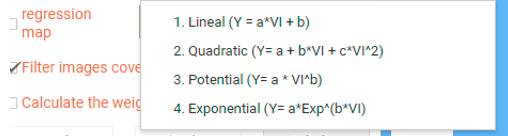
\includegraphics{./images/Figure8} 

}

\caption{Funciones consideradas}\label{fig:figG8}
\end{figure}

\emph{\textbf{iii) Filtrar imágenes que cubran todo el polígono:} cuando se active esta opción se filtrar imágenes que cubran completamente el polígono(s) de la zona, de otra manera, se muestra imágenes aunque cubran un cierto porcentaje de la zona. Esta opción es útil para polígonos que abarcan superficies grandes (cientos de has).}\\
\emph{\textbf{iv) Calcular factor de ponderación:} Es la relación entre el valor del índice en un píxel y el promedio del índice en el polígono (parcela). Se calcula por cada polígono digitalizado. Este factor en una parcela agrícola es un indicador normalizado del potencial productivo de cada píxel de una imagen. }

\textbf{5) Calcular: }: Cuando se tenga configurado las opciones se debe dar clic en \textbf{calculate} y se mostraran mínimo tres capas en el mapa: \emph{\textbf{i) imagen RGB de la primera imagen encontrada en el intervalo establecido, ii) índices de vegetación}. }

\hypertarget{usando-poligonos-digitalizados}{%
\section{Usando poligonos digitalizados}\label{usando-poligonos-digitalizados}}

EL usuario puede digitalizar cualquier parcela (polígonos) usando las herramientas de dibujo que se encuentran en la esquina superior izquierda del mapa (Figura \ref{fig:figG9}). El programa reconoce que se deben calcular los índices de vegetación sobre estos polígonos.

\begin{figure}

{\centering 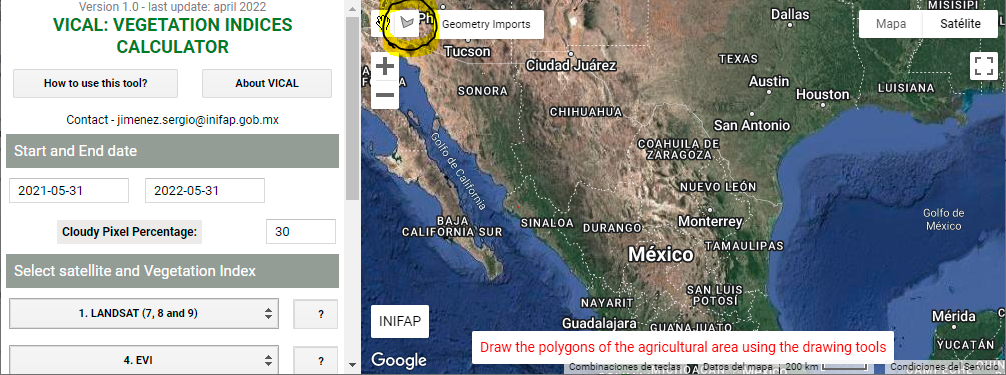
\includegraphics[width=0.75\linewidth]{./images/Figure11} 

}

\caption{Herramientas de dibujo}\label{fig:figG9}
\end{figure}

Esta opción es útil cuando son pocas parcelas donde se desea estimar IVs (Figura \ref{fig:figG10}). O bien, también es útil cuando se desea descargar índices de vegetación de una zona en particular sin importar los limites parcelarios (Figura \ref{fig:figG11}).

Para editar el polígono o crear un nuevo polígono se debe dar clic en los botones \emph{``Edit y New Polygon''} respectivamente. Estas opciones están disponibles después de que se ha realizado un calculo.

\begin{figure}

{\centering 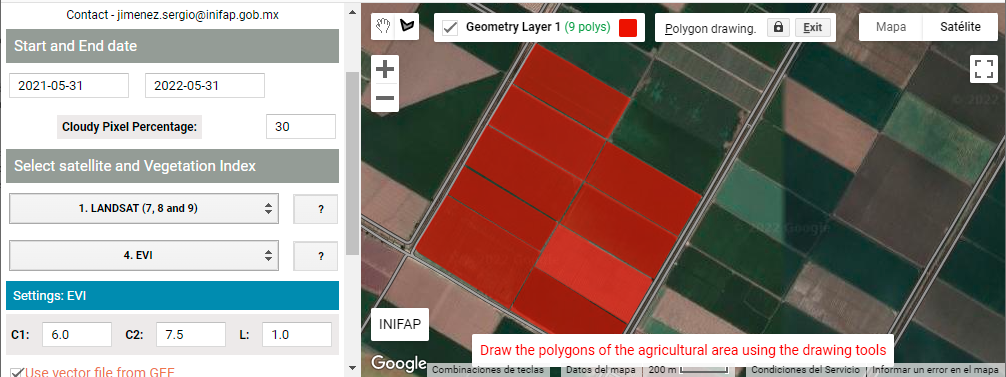
\includegraphics[width=0.75\linewidth]{./images/Figure12} 

}

\caption{Parcelas digitalizadas}\label{fig:figG10}
\end{figure}

\begin{figure}

{\centering 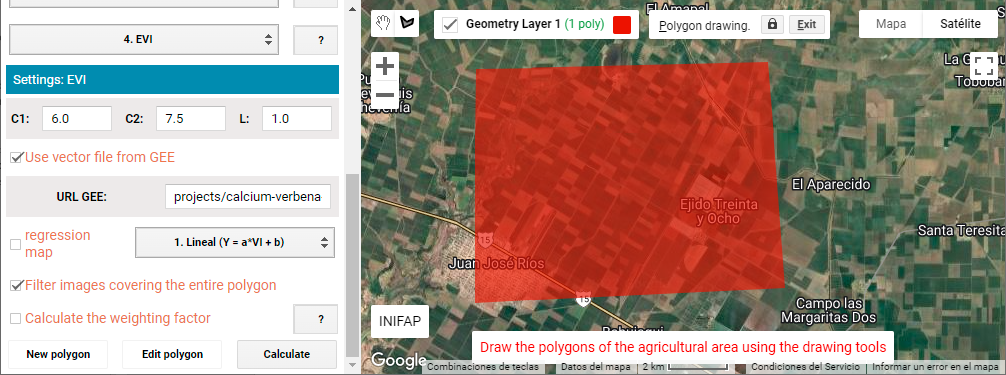
\includegraphics[width=0.75\linewidth]{./images/Figure13} 

}

\caption{poligono digitalizados}\label{fig:figG11}
\end{figure}

\hypertarget{usando-archivo-vector}{%
\section{Usando archivo vector}\label{usando-archivo-vector}}

Para esta opción, el usuario debe ingresar el \textbf{URL} del archivo vector con el que desea realizar los cálculos; esto indica que debe tener una cuenta en GEE e importar un archivo vector tipo polígono en su cuenta.

La URL se puede obtener dando clic izquierdo sobre el archivo que se encuentra en la pestalla \emph{\textbf{Assets}} de su cuenta de GEE (Figura \ref{fig:figG12}).

\begin{figure}

{\centering 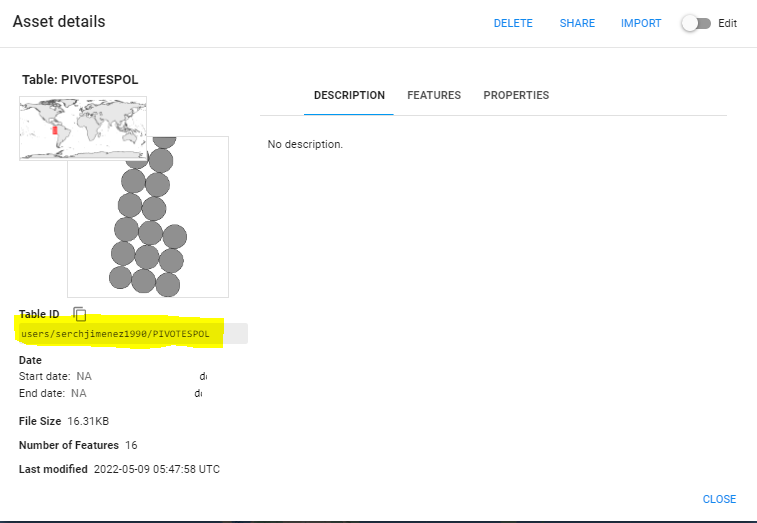
\includegraphics[width=0.75\linewidth]{./images/Figure14} 

}

\caption{detalles en GEE del archivo vector}\label{fig:figG12}
\end{figure}

Una cuestión importante, para que el archivo vector se puede emplear en \textbf{VICAL} debe tener tener activado la casilla ``Anyone can read'' (Figura \ref{fig:figG13}).

\begin{figure}

{\centering 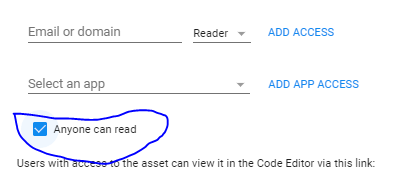
\includegraphics[width=0.75\linewidth]{./images/Figure6} 

}

\caption{poligono digitalizadas}\label{fig:figG13}
\end{figure}

\hypertarget{implementaciuxf3n}{%
\chapter{Implementación}\label{implementaciuxf3n}}

En esta sección se presenta un ejemplo de como navegar en dicha aplicación y como muestra los resultados VICAL.

\hypertarget{PriVis}{%
\section{Primeras visualizaciones}\label{PriVis}}

Cuando los índices de vegetación (IV) se calculan usando VICAL, se muestran mínimo tres capas obligatorias y otras opcionales: (i) combinación RGB \emph{(Figura \ref{fig:figI1})}, (ii) el IV seleccionado \emph{(Figura \ref{fig:figI2})}, (iii) factor de ponderación (opcional) calculado por cada polígono \emph{(Figura \ref{fig:figI3})}, (iv) el mapa de regresión \emph{(Figura \ref{fig:figI4})} y (v) polígonos dibujados por el usuario. Estos mapas, en principio, son obtenidos a partir de la primera imagen encontrada de la coleccion de imagenes.

En las siguientes imágenes se muestran algunas visualizaciones obtenidas a partir de la URL que viene por defecto en VICAL y se activó la casilla \emph{``Use vector file from GEE''} y activando la opción de \emph{regresión lineal} con coeficientes de a=1.15 y b=0.17.

\begin{figure}

{\centering 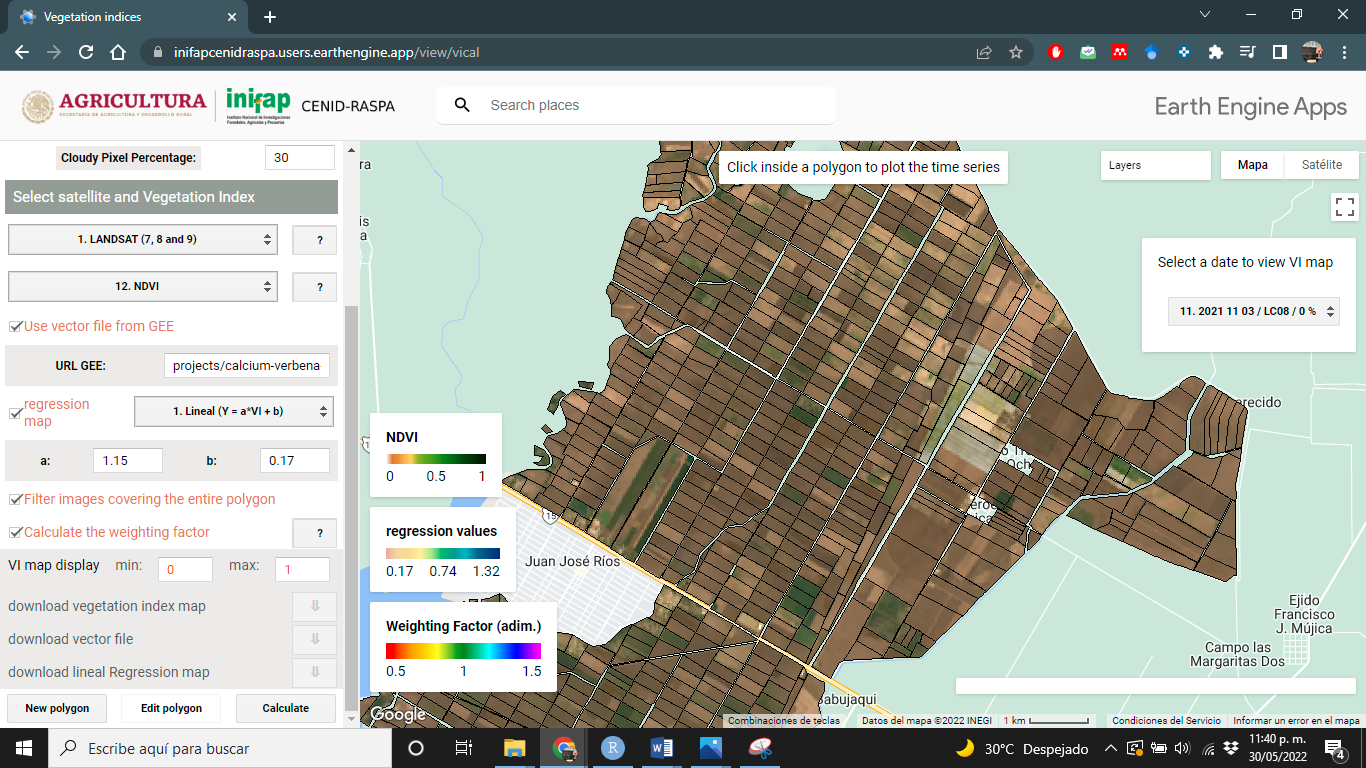
\includegraphics[width=0.85\linewidth]{./images/Figure51} 

}

\caption{Combinacion RGB}\label{fig:figI1}
\end{figure}

\begin{figure}

{\centering 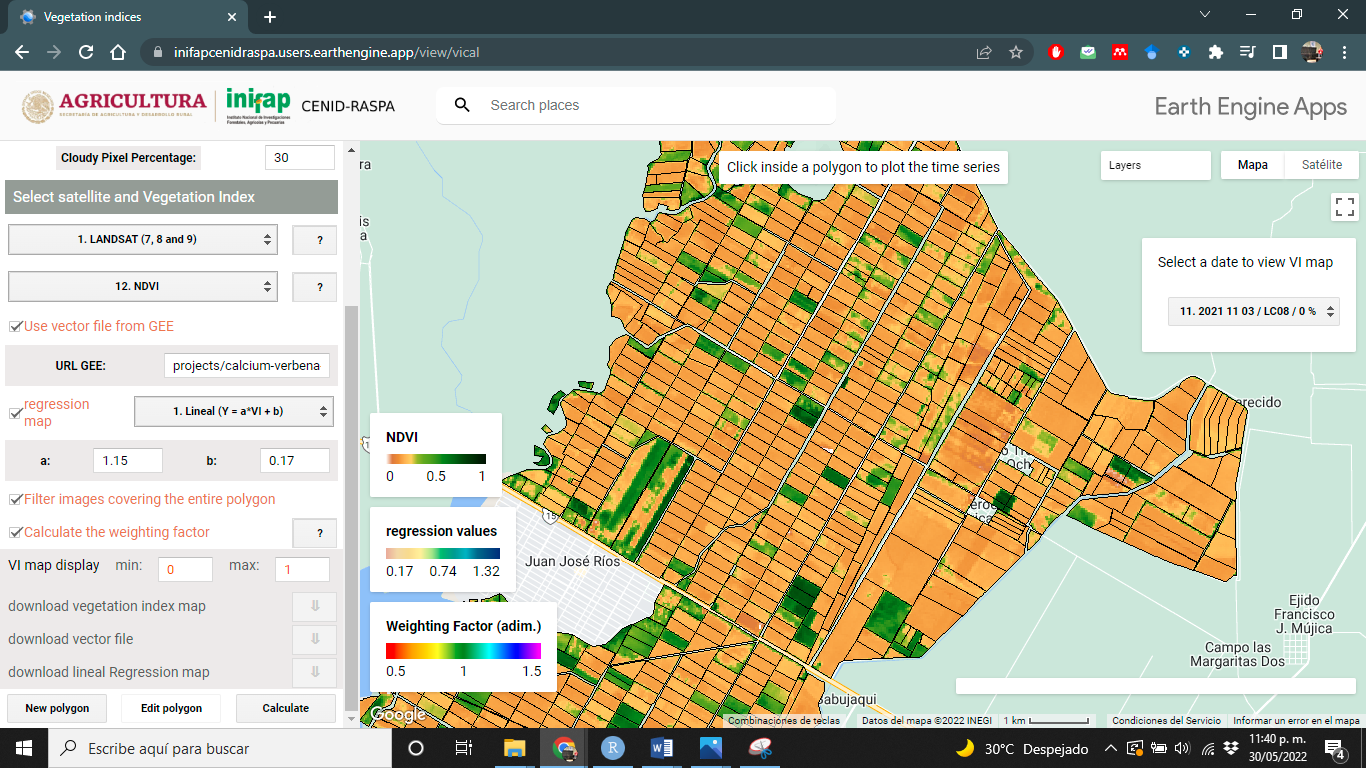
\includegraphics[width=0.85\linewidth]{./images/Figure52} 

}

\caption{mapa de NDVI}\label{fig:figI2}
\end{figure}

\begin{figure}

{\centering 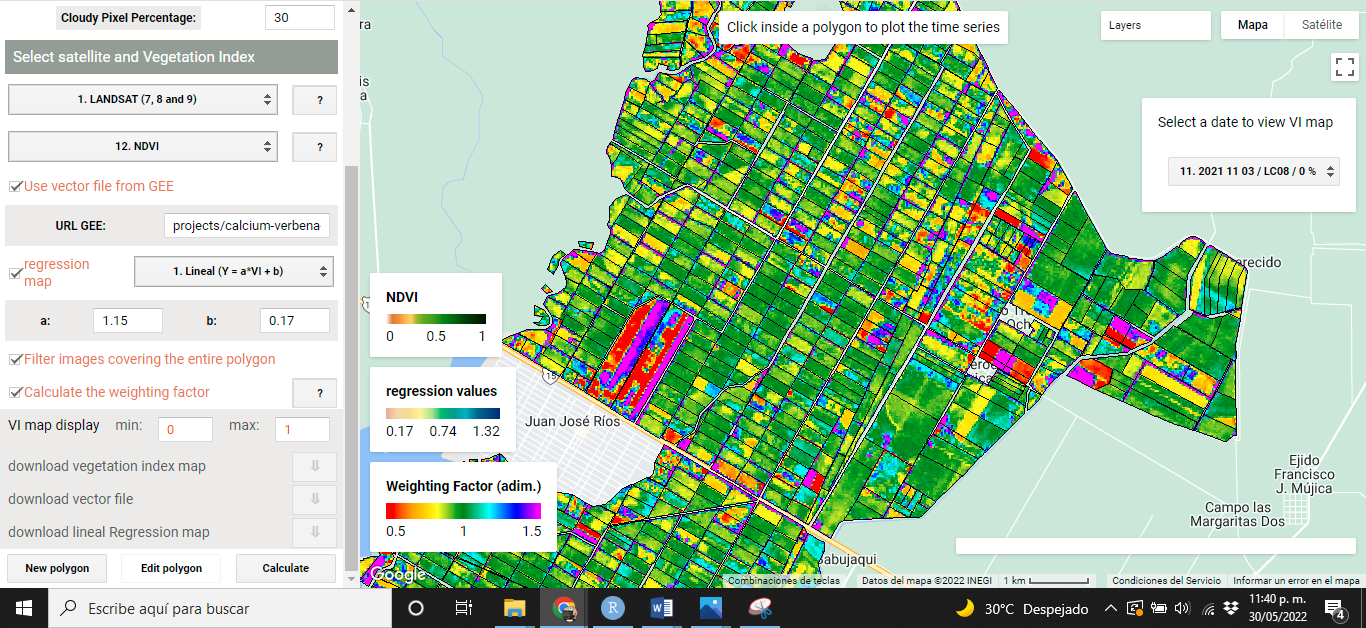
\includegraphics[width=0.85\linewidth]{./images/Figure53} 

}

\caption{Factor de ponderación (opcional)}\label{fig:figI3}
\end{figure}

\begin{figure}

{\centering 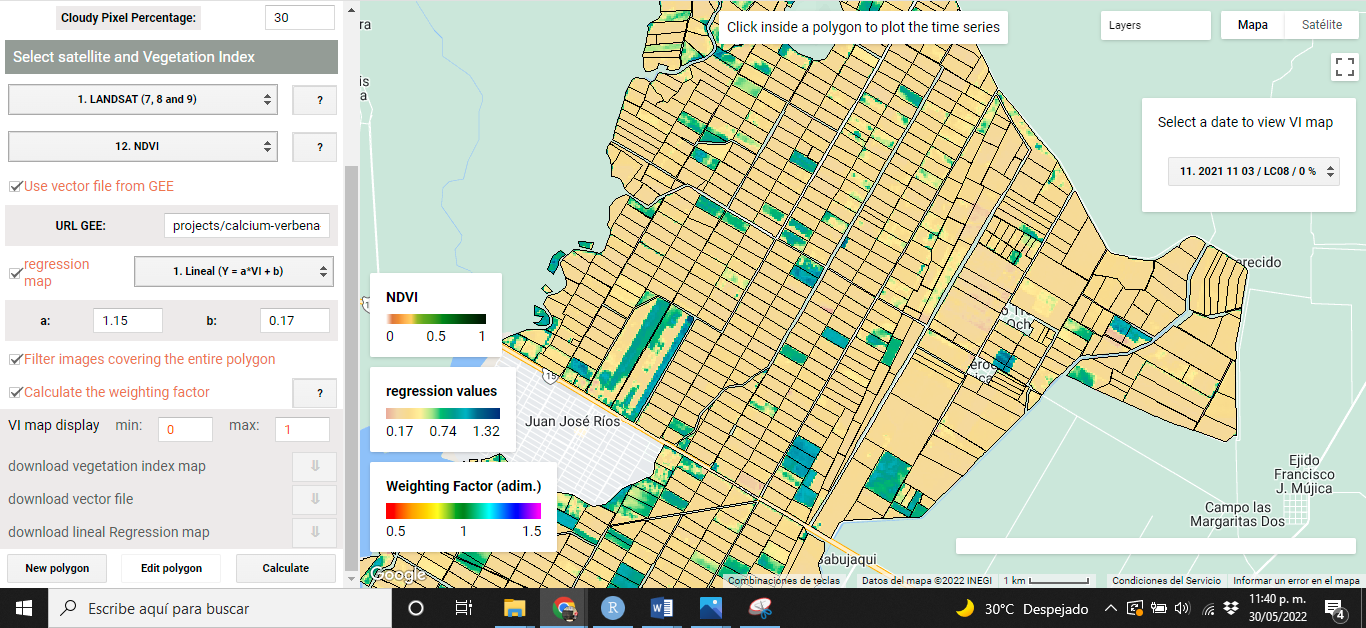
\includegraphics[width=0.85\linewidth]{./images/Figure54} 

}

\caption{Mapa de Regresión (opcional)}\label{fig:figI4}
\end{figure}

\hypertarget{navegar-entre-imagenes}{%
\section{Navegar entre imagenes}\label{navegar-entre-imagenes}}

El programa crea una colección de imágenes definida por la configuración del usuario; el usuario puede navegar entre las imágenes encontradas, para ello, del lado superior derecho aparece una barra en donde al dar clic despliega unas filas donde cada una representa una imagen.

La nomenclatura corta que se empleó para nombrar las imágenes son (Figura \ref{fig:figI5}): \emph{Número de imagen encontrada \textbf{+} punto \textbf{+} Fecha de la imagen (comenzando por año, mes y día) \textbf{+} / \textbf{+} Sensor \textbf{+} / \textbf{+} Porcentaje de nubes en la imagen.}

\begin{figure}

{\centering 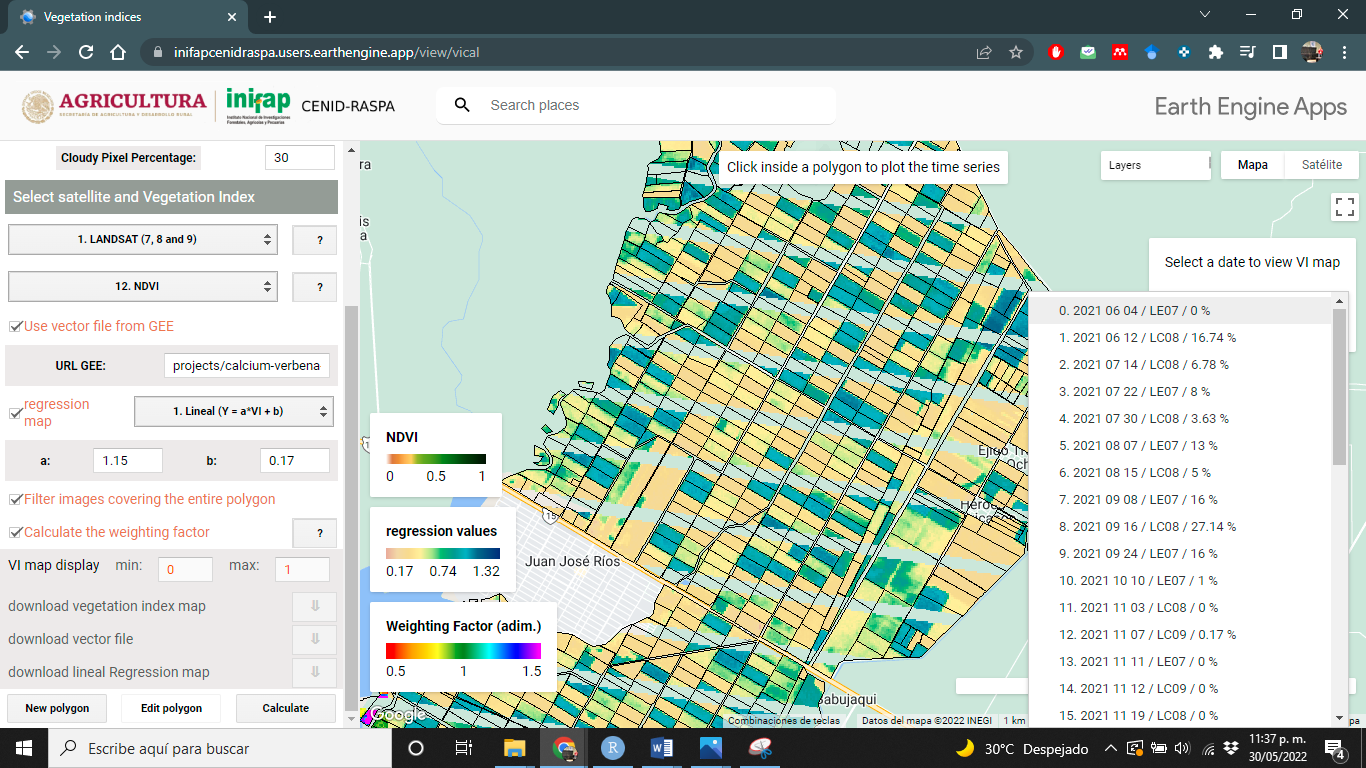
\includegraphics[width=0.85\linewidth]{./images/Figure55} 

}

\caption{Lista de imagenes encontradas}\label{fig:figI5}
\end{figure}

Se debe dar clic en cualquier imagen que se desea visualizar y apareceran las capas descritas en la sección \ref{PriVis} para la imagen seleccionada (Figura \ref{fig:figI6}).

\begin{figure}

{\centering 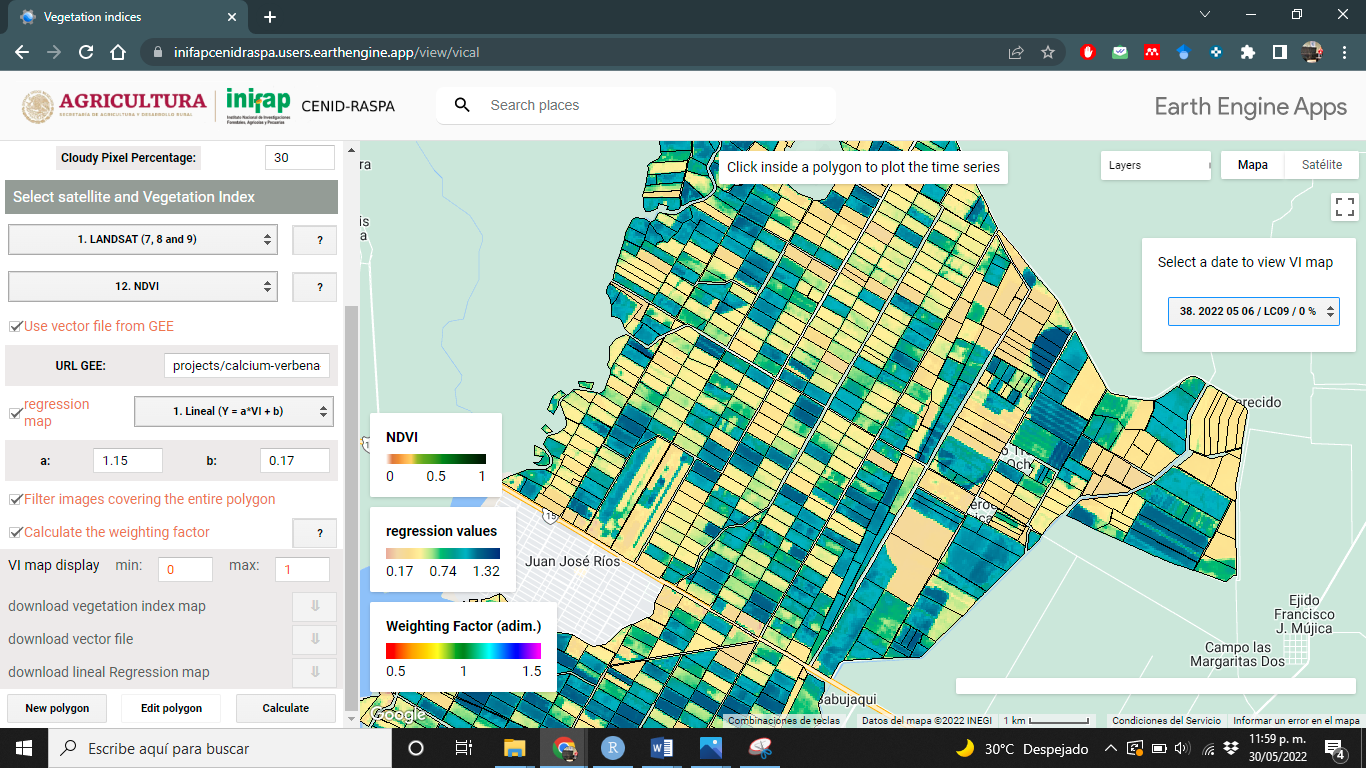
\includegraphics[width=0.85\linewidth]{./images/Figure56} 

}

\caption{Mapas para fecha seleccionada}\label{fig:figI6}
\end{figure}

\hypertarget{visualizaciuxf3n-del-mapa-de-iv}{%
\section{Visualización del mapa de IV}\label{visualizaciuxf3n-del-mapa-de-iv}}

El usuario puede cambiar los valores de visualización del mapa de IV cambiando el rango en que varia el valor \textbf{máximo} y \textbf{mínimo}, para ello debe ingresar los valores en la opción \emph{``VI map display''} (Figura \ref{fig:figI7}) y presionar la tecla Enter con el teclado.

\begin{figure}

{\centering 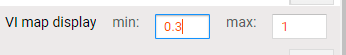
\includegraphics{./images/Figure57} 

}

\caption{Ajuste de visualiacion del mapa de IV}\label{fig:figI7}
\end{figure}

El programa reconoce cuando se cambia el valor y automáticamente crea la capa con la nueva visualización (Figura \ref{fig:figI8}). Es posible cambiar estos valores de visualización después de que el usuario haya navegado entre imágenes.

\begin{figure}

{\centering 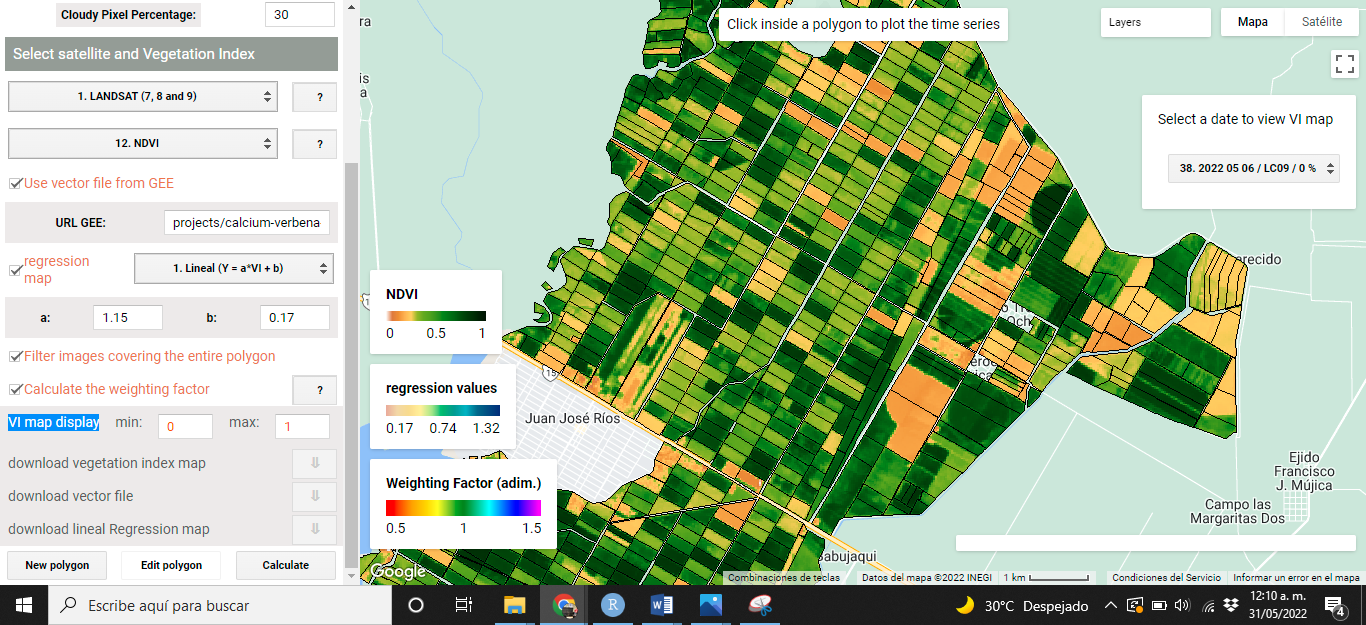
\includegraphics[width=0.85\linewidth]{./images/Figure58} 

}

\caption{NDVI con valores en el rango [0,1]}\label{fig:figI8}
\end{figure}

\begin{figure}

{\centering 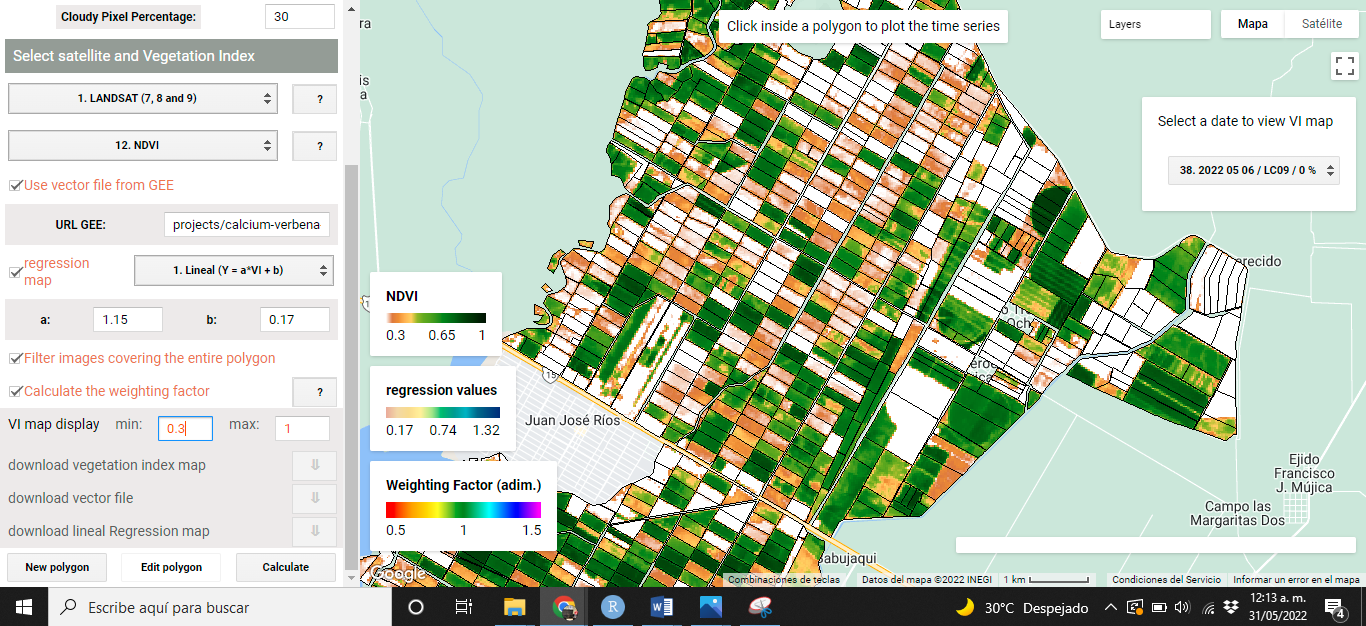
\includegraphics[width=0.85\linewidth]{./images/Figure59} 

}

\caption{NDVI con valores en el rango [0.3,1]}\label{fig:figI9}
\end{figure}

\hypertarget{series-de-tiempo}{%
\section{Series de tiempo}\label{series-de-tiempo}}

La serie de tiempo del IV se obtiene al dar clic sobre cualquier polígono, por tanto, los valores son únicamente del polígono seleccionado. La serie de tiempo se muestra en una gráfica donde se calcula el promedio y desviación estándar de los valores del IV, cada punto representa una imagen encontrada según la configuración del usuario (Figura \ref{fig:figI10} y (Figura \ref{fig:figI11})).

\begin{figure}

{\centering 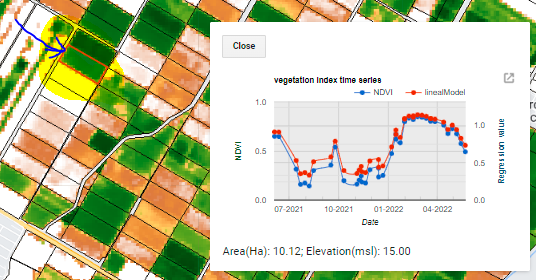
\includegraphics{./images/Figure60} 

}

\caption{Serie de tiempo del IV para la parcela indicada}\label{fig:figI10}
\end{figure}
\begin{figure}

{\centering 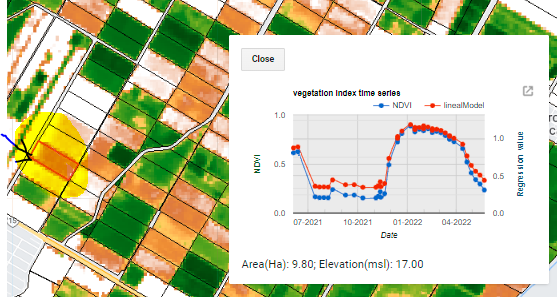
\includegraphics{./images/Figure61} 

}

\caption{Serie de tiempo del IV para la parcela indicada}\label{fig:figI11}
\end{figure}

\hypertarget{descargar-informaciuxf3n}{%
\section{Descargar información}\label{descargar-informaciuxf3n}}

Se pueden descargar tres capas de las cinco que se muestran en el mapa. Estas opciones (botones) se muestran en la parte inferior de la sección de configuración (Figura \ref{fig:figI12}). Las capas que se permiten descargar son:

\begin{figure}

{\centering 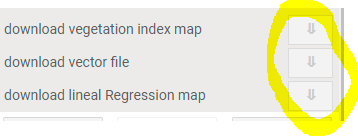
\includegraphics{./images/Figure62} 

}

\caption{opciones de descarga}\label{fig:figI12}
\end{figure}

\textbf{i) Mapa de vegetación:} Se descarga la imagen Raster con valores del índice de vegetación calculada y recortada para la zona de interés, la descarga se realiza en formato TIF que puede ser visualizado por ejemplo en QGIS \emph{(Figura \ref{fig:figI13})}.

\textbf{ii) Archivo vector:} Se descarga el polígono digitalizado o bien el archivo vector en formato kml, que puede ser visualizado por ejemplo en Google Earth.

\textbf{iii) Mapa de regresión:} Esta opción está disponible si se activa la casilla de ``regression map'', se descarga la imagen raster con valores del mapa de regresión y recortada para la zona de interés, la descarga se realiza en formato TIF que puede ser visualizado por ejemplo en QGIS.

\begin{figure}

{\centering 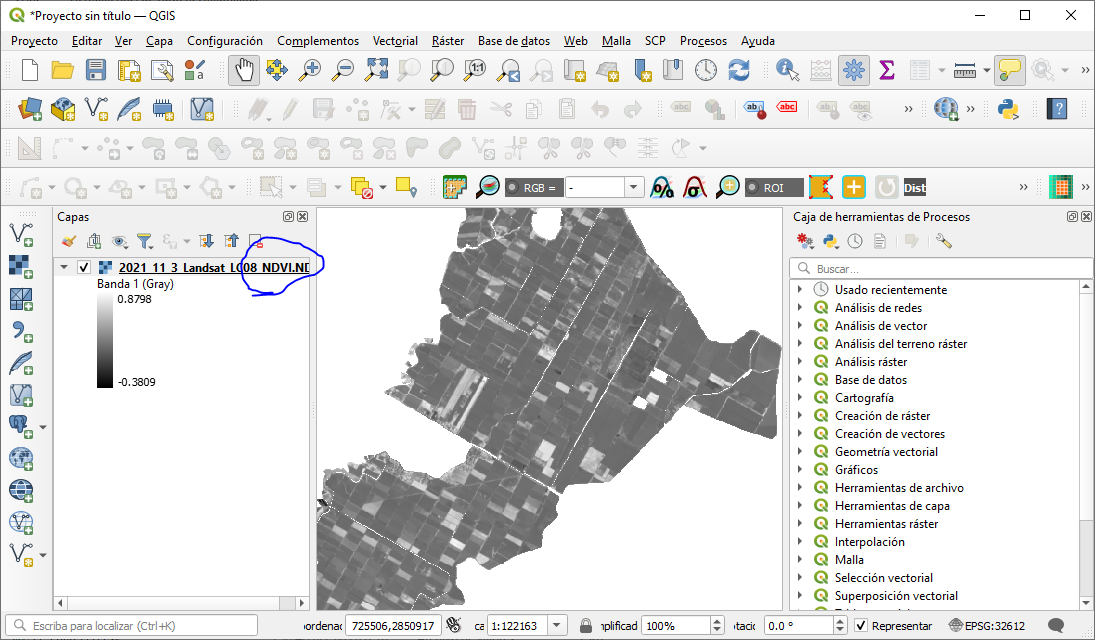
\includegraphics[width=0.85\linewidth]{./images/Figure63} 

}

\caption{Imagen de NDVI visualizado en QGIS}\label{fig:figI13}
\end{figure}

\hypertarget{vical-en-gee}{%
\chapter{VICAL en GEE}\label{vical-en-gee}}

En esta sección se muestra cómo usar los archivos de VICAL para implementarlos en un script propio de GEE.

VICAL cuenta con tres archivos que puede importar a su Script, estos son:

\begin{Shaded}
\begin{Highlighting}[]
\CommentTok{// archivo para las colecciones de imagenes);}
\KeywordTok{var}\NormalTok{ imp }\OperatorTok{=} \PreprocessorTok{require}\NormalTok{(}\StringTok{\textquotesingle{}users/InifapCenidRaspa/VICAL:Exportaciones\textquotesingle{}}\NormalTok{)}\OperatorTok{;}
\CommentTok{// archivo para los indices de vegetacion}
\KeywordTok{var}\NormalTok{ imp2}\OperatorTok{=} \PreprocessorTok{require}\NormalTok{(}\StringTok{\textquotesingle{}users/InifapCenidRaspa/VICAL:VegetationIndex\textquotesingle{}}\NormalTok{)}\OperatorTok{;} 
\CommentTok{// archivo para las visualizaciones}
\KeywordTok{var}\NormalTok{ St}\OperatorTok{=} \PreprocessorTok{require}\NormalTok{(}\StringTok{\textquotesingle{}users/InifapCenidRaspa/VICAL:Style\textquotesingle{}}\NormalTok{)}\OperatorTok{;}
\end{Highlighting}
\end{Shaded}

\hypertarget{CImg}{%
\section{Coleccion de imagenes}\label{CImg}}

Antes de importar el conjunto de colecciones de imágenes se deben definir ciertas variables que van a ser útiles para filtrar la colección, estos son: i) un punto o polígono; ii) intervalo de fechas y iii) valor umbral de nubes en las imágenes; esto se muestra a continuación:

\begin{Shaded}
\begin{Highlighting}[]
\KeywordTok{var}\NormalTok{ fecha }\OperatorTok{=}\NormalTok{ [}\StringTok{\textquotesingle{}2021{-}01{-}01\textquotesingle{}}\OperatorTok{,} \StringTok{\textquotesingle{}2022{-}03{-}18\textquotesingle{}}\NormalTok{]}\OperatorTok{;} \CommentTok{//Fecha inicial y final }
\CommentTok{//poligono o punto}
\KeywordTok{var}\NormalTok{ table }\OperatorTok{=}\NormalTok{ ee}\OperatorTok{.}\FunctionTok{FeatureCollection}\NormalTok{(}\StringTok{"projects/calcium{-}verbena{-}328905/assets/Bate"}\NormalTok{)}\OperatorTok{;} 
\KeywordTok{var}\NormalTok{ p\_nubes}\OperatorTok{=} \DecValTok{30}\OperatorTok{;}\CommentTok{//Porcentaje de nubes}
\end{Highlighting}
\end{Shaded}

\hypertarget{landsat}{%
\subsection{Landsat}\label{landsat}}

Si se desea usar imágenes LandSat (4, 5, 7, 8 y 9) corregidas atmosféricamente libre de nubes se puede usar el código siguiente, donde se crea una función para unir las colecciones de imágenes. Para ello se usa el archivo \textbf{\emph{imp}}.

\begin{Shaded}
\begin{Highlighting}[]
\KeywordTok{function} \FunctionTok{ColeccionImagenSR}\NormalTok{(fecha}\OperatorTok{,}\NormalTok{ recorte}\OperatorTok{,}\NormalTok{ umbral)}
\NormalTok{\{}
  \CommentTok{// se importan las colecciones de imagenes usando el archivo "imp"}
  \KeywordTok{var}\NormalTok{ L9sr }\OperatorTok{=}\NormalTok{ imp}\OperatorTok{.}\FunctionTok{ColeccionLandsatSR}\NormalTok{(fecha}\OperatorTok{,} \StringTok{\textquotesingle{}LC09\textquotesingle{}}\OperatorTok{,}\NormalTok{ recorte}\OperatorTok{,}\NormalTok{ umbral)}\OperatorTok{;}
  \KeywordTok{var}\NormalTok{ L8sr }\OperatorTok{=}\NormalTok{ imp}\OperatorTok{.}\FunctionTok{ColeccionLandsatSR}\NormalTok{(fecha}\OperatorTok{,} \StringTok{\textquotesingle{}LC08\textquotesingle{}}\OperatorTok{,}\NormalTok{ recorte}\OperatorTok{,}\NormalTok{ umbral)}\OperatorTok{;}
  \KeywordTok{var}\NormalTok{ L7sr }\OperatorTok{=}\NormalTok{ imp}\OperatorTok{.}\FunctionTok{ColeccionLandsatSR}\NormalTok{(fecha}\OperatorTok{,} \StringTok{\textquotesingle{}LE07\textquotesingle{}}\OperatorTok{,}\NormalTok{ recorte}\OperatorTok{,}\NormalTok{ umbral)}\OperatorTok{;}
  \KeywordTok{var}\NormalTok{ L5sr }\OperatorTok{=}\NormalTok{ imp}\OperatorTok{.}\FunctionTok{ColeccionLandsatSR}\NormalTok{(fecha}\OperatorTok{,} \StringTok{\textquotesingle{}LT05\textquotesingle{}}\OperatorTok{,}\NormalTok{ recorte}\OperatorTok{,}\NormalTok{ umbral)}\OperatorTok{;}
  \KeywordTok{var}\NormalTok{ L4sr }\OperatorTok{=}\NormalTok{ imp}\OperatorTok{.}\FunctionTok{ColeccionLandsatSR}\NormalTok{(fecha}\OperatorTok{,} \StringTok{\textquotesingle{}LT04\textquotesingle{}}\OperatorTok{,}\NormalTok{ recorte}\OperatorTok{,}\NormalTok{ umbral)}\OperatorTok{;}
  \CommentTok{//Los datos de ETM y ETM+ se ajustan espectrales a OLI y OLI{-}2 }
  \KeywordTok{var}\NormalTok{ L7a }\OperatorTok{=}\NormalTok{ L7sr}\OperatorTok{.}\FunctionTok{map}\NormalTok{(imp}\OperatorTok{.}\AttributeTok{TMaOLI}\NormalTok{)}\OperatorTok{;}
  \KeywordTok{var}\NormalTok{ L5a }\OperatorTok{=}\NormalTok{ L5sr}\OperatorTok{.}\FunctionTok{map}\NormalTok{(imp}\OperatorTok{.}\AttributeTok{TMaOLI}\NormalTok{)}\OperatorTok{;}
  \KeywordTok{var}\NormalTok{ L4a }\OperatorTok{=}\NormalTok{ L4sr}\OperatorTok{.}\FunctionTok{map}\NormalTok{(imp}\OperatorTok{.}\AttributeTok{TMaOLI}\NormalTok{)}\OperatorTok{;}
  \CommentTok{// Une las tres series de imágenes}
  \KeywordTok{var}\NormalTok{ serieT }\OperatorTok{=}\NormalTok{L9sr}\OperatorTok{.}\FunctionTok{merge}\NormalTok{(L8sr)}\OperatorTok{.}\FunctionTok{merge}\NormalTok{(L7a)}\OperatorTok{.}\FunctionTok{merge}\NormalTok{(L5a)}\OperatorTok{.}\FunctionTok{merge}\NormalTok{(L4a)}\OperatorTok{.}\FunctionTok{sort}\NormalTok{(}\StringTok{\textquotesingle{}system:time\_start\textquotesingle{}}\NormalTok{)}\OperatorTok{;}
    \ControlFlowTok{return}\NormalTok{ serieT}\OperatorTok{;}
\NormalTok{\}}
\CommentTok{//SE importa la coleccion usando la funccion anterior }
\KeywordTok{var}\NormalTok{ l8Sergio}\OperatorTok{=}\FunctionTok{ColeccionImagenSR}\NormalTok{(fecha}\OperatorTok{,}\NormalTok{ table}\OperatorTok{,}\NormalTok{ p\_nubes)}\OperatorTok{;}
\CommentTok{//podemos imprimir las imagenes usando la funcion print() para ver }
\CommentTok{//si se llevo a cabo el filtrado de la coleccion de imagenes (Figura 6.1) }
\FunctionTok{print}\NormalTok{ (l8Sergio)}\OperatorTok{;}
\end{Highlighting}
\end{Shaded}

Con estas colecciones de imágenes se pueden calcular series de tiempo de diferentes índices de vegetación.

\begin{figure}

{\centering 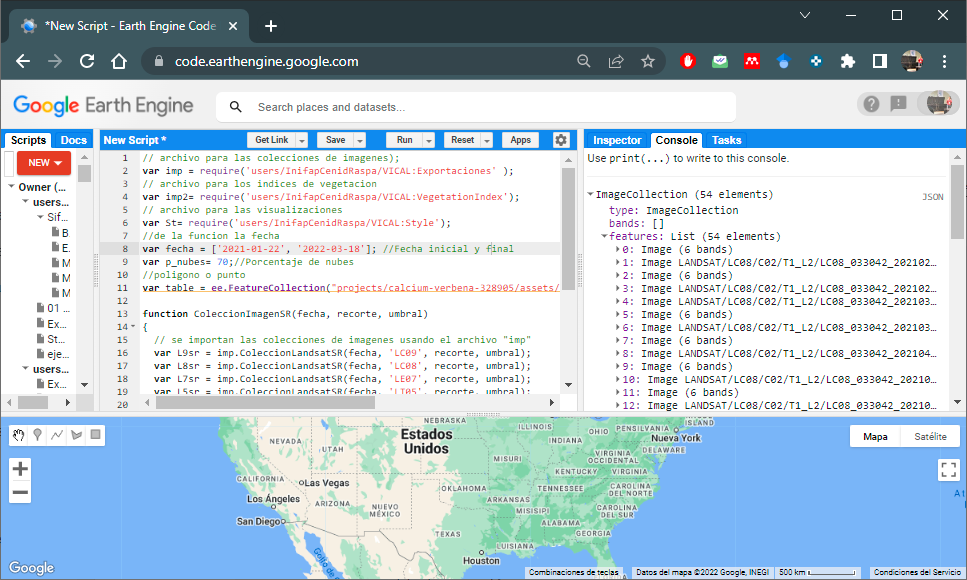
\includegraphics[width=0.85\linewidth]{./images/Figure70} 

}

\caption{Impresion de coleccion de imagenes Landsat}\label{fig:figV1}
\end{figure}

\hypertarget{sentinel-2}{%
\subsection{Sentinel-2}\label{sentinel-2}}

Si se desea usar imágenes Sentinel-2 corregidas atmosféricamente libre de nubes se puede usar el siguiente código.

\begin{Shaded}
\begin{Highlighting}[]
\CommentTok{//SE importa la coleccion usando el siguiente codigo}
\KeywordTok{var}\NormalTok{ S2sr }\OperatorTok{=}\NormalTok{ imp}\OperatorTok{.}\FunctionTok{ColeccionImagenSentinelSR}\NormalTok{(fecha}\OperatorTok{,}\NormalTok{ table}\OperatorTok{,}\NormalTok{ p\_nubes)}\OperatorTok{;}
\CommentTok{//podemos imprimir las imagenes usando la funcion print() para ver }
\CommentTok{//si se llevo a cabo el filtrado de la coleccion de imagenes (Figura 6.2)}
\FunctionTok{print}\NormalTok{ (S2sr)}\OperatorTok{;}
\end{Highlighting}
\end{Shaded}

\begin{figure}

{\centering 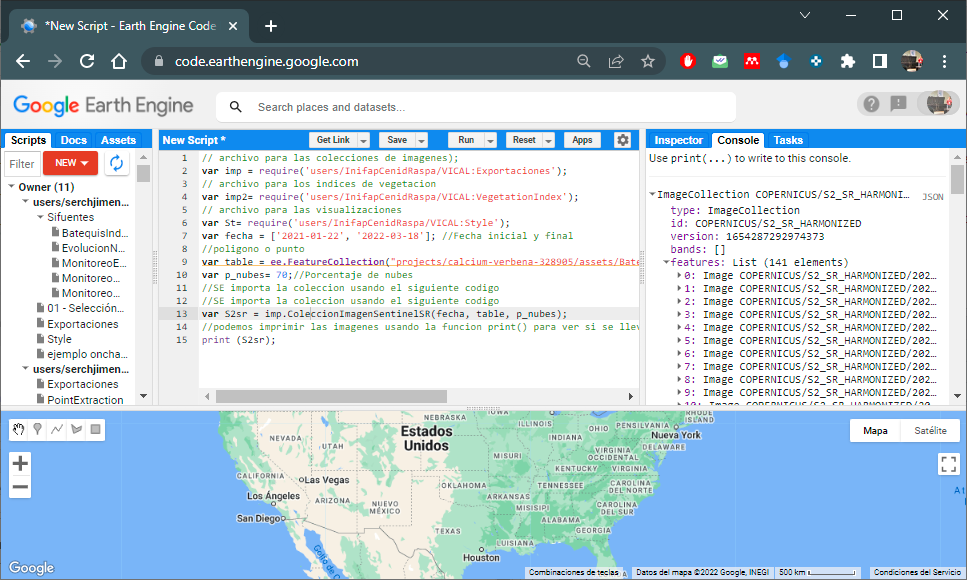
\includegraphics[width=0.85\linewidth]{./images/Figure71} 

}

\caption{Impresion de coleccion de imagenes Sentinel-2}\label{fig:figV2}
\end{figure}

\hypertarget{LanSen}{%
\subsection{Landsat y Sentinel-2}\label{LanSen}}

Si se desea usar imágenes LandSat y Sentinel-2 corregidas atmosféricamente libre de nubes se puede usar el siguiente código, los datos se ajustaron espectralmente a las bandas espectrales de Landsat 8. Se emplean las funciones descritas en la Sección \ref{CImg}:

\begin{Shaded}
\begin{Highlighting}[]
\KeywordTok{function} \FunctionTok{ColeccionImagenAMBOS}\NormalTok{(fecha}\OperatorTok{,}\NormalTok{ recorte}\OperatorTok{,}\NormalTok{ umbral)}
\NormalTok{\{}
  \CommentTok{//Se lee la function para imagenes Landsat con ajuste espectral}
  \KeywordTok{var}\NormalTok{ L8Conjunto}\OperatorTok{=}\FunctionTok{ColeccionImagenSR}\NormalTok{(fecha}\OperatorTok{,}\NormalTok{ recorte}\OperatorTok{,}\NormalTok{ umbral)}
  \CommentTok{//coleccion sentinel}
  \KeywordTok{var}\NormalTok{ S2sr }\OperatorTok{=}\NormalTok{ imp}\OperatorTok{.}\FunctionTok{ColeccionImagenSentinelSR}\NormalTok{(fecha}\OperatorTok{,}\NormalTok{ recorte}\OperatorTok{,}\NormalTok{ umbral)}\OperatorTok{;}
  \KeywordTok{var}\NormalTok{ S2a }\OperatorTok{=}\NormalTok{ S2sr}\OperatorTok{.}\FunctionTok{map}\NormalTok{(imp}\OperatorTok{.}\AttributeTok{MSIaOLI}\NormalTok{)}\OperatorTok{;} \CommentTok{//Se hace el ajuste espectral de sentinel{-}2 a Landsat}
  \KeywordTok{var}\NormalTok{ serieT }\OperatorTok{=}\NormalTok{ S2a}\OperatorTok{.}\FunctionTok{merge}\NormalTok{(L8Conjunto)}\OperatorTok{.}\FunctionTok{sort}\NormalTok{(}\StringTok{\textquotesingle{}system:time\_start\textquotesingle{}}\NormalTok{)}\OperatorTok{;}
    \ControlFlowTok{return}\NormalTok{ serieT}\OperatorTok{;}
\NormalTok{\}}

\CommentTok{//SE importa la coleccion usando el siguiente codigo}
\KeywordTok{var}\NormalTok{ S2B }\OperatorTok{=} \FunctionTok{ColeccionImagenAMBOS}\NormalTok{(fecha}\OperatorTok{,}\NormalTok{ table}\OperatorTok{,}\NormalTok{ p\_nubes)}\OperatorTok{;}
\CommentTok{//podemos imprimir las imagenes usando la funcion print() para ver }
\CommentTok{//si se llevo a cabo el filtrado de la coleccion de imagenes (Figura 6.3)}
\FunctionTok{print}\NormalTok{ (S2sr)}\OperatorTok{;}
\end{Highlighting}
\end{Shaded}

\begin{figure}

{\centering 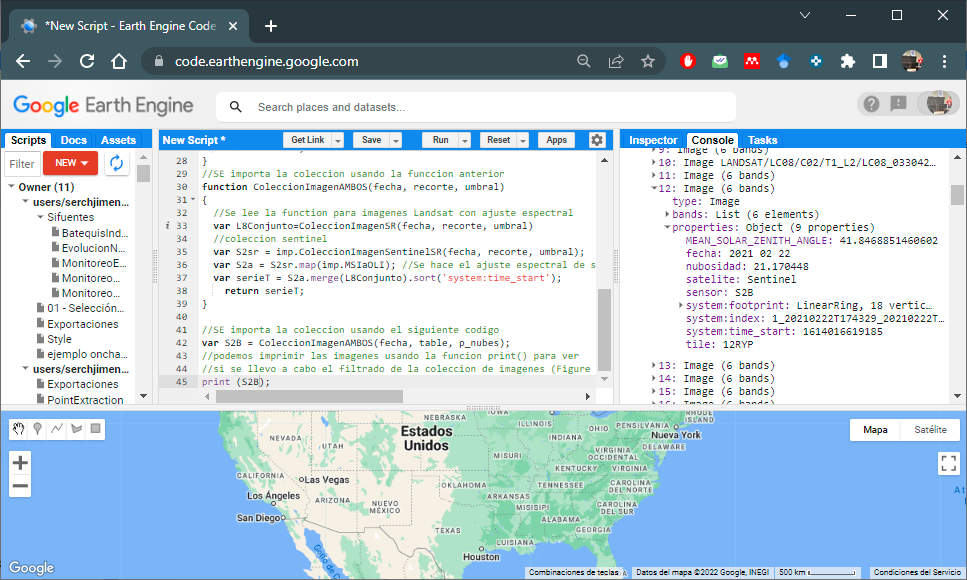
\includegraphics[width=0.85\linewidth]{./images/Figure72} 

}

\caption{Impresion de coleccion de imagenes Landsat y Sentinel-2}\label{fig:figV3}
\end{figure}

Para revisar un Script de ejemplo clic \href{https://code.earthengine.google.com/1eb76041c45bccf238c28ee9a4bad955}{aquí}

\hypertarget{indices-de-vegetaciuxf3n}{%
\section{Indices de vegetación}\label{indices-de-vegetaciuxf3n}}

Para usar el código de índices de vegetación de \textbf{VICAL} se tienen que usar el archivo \textbf{imp2}; y se mandan a llamar estos IV usando los nombres de la columna \textbf{ExpresionGEE} que se muestran en la \textbf{Tabla \ref{tab:Index}}.

Por ejemplo, para calcular el NDVI con la colección de imágenes LandSat y Sentinel-2 de la sección \ref{LanSen} se usaría el siguiente código:

\begin{Shaded}
\begin{Highlighting}[]
\CommentTok{//Normalized Difference Vegetation Index{-} NDVI}
\KeywordTok{var}\NormalTok{ ivs }\OperatorTok{=}\NormalTok{ ee}\OperatorTok{.}\FunctionTok{ImageCollection}\NormalTok{(S2B}\OperatorTok{.}\FunctionTok{map}\NormalTok{(imp2}\OperatorTok{.}\AttributeTok{NDVI}\NormalTok{))}\OperatorTok{;}
\CommentTok{//para imprimir y ver la banda de NDVI}
\FunctionTok{print}\NormalTok{ (ivs)}\OperatorTok{;}
\end{Highlighting}
\end{Shaded}

En la Figura \ref{fig:figV4} se muestra que en la colección de imágenes del conjunto armonizado aparece una sola banda que se llama \textbf{NDVI}.

\begin{figure}

{\centering 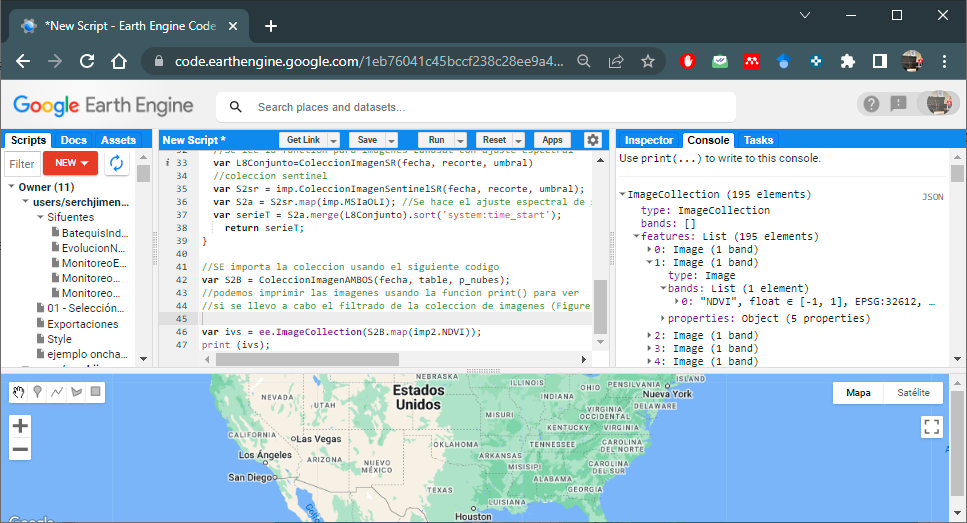
\includegraphics[width=0.85\linewidth]{./images/Figure73} 

}

\caption{Impresion de coleccion de imagenes con banda NDVI}\label{fig:figV4}
\end{figure}

Ahora, para visualizar en el mapa el \textbf{NDVI} de la primera imagen de la colección y recortado para la zona quedaría como se muestra en el código siguiente; donde para ver la paleta de colores se utilizaría el archivo \textbf{st } de ¨\textbf{VICAL}.

\begin{Shaded}
\begin{Highlighting}[]
\CommentTok{//Se obtiene el NDVI de la primera imagen en la coleccion }
\KeywordTok{var}\NormalTok{ iv }\OperatorTok{=}\NormalTok{ ivs}\OperatorTok{.}\FunctionTok{first}\NormalTok{()}\OperatorTok{;}
\CommentTok{//Paleta de colores donde se usa el archivo st}
\KeywordTok{var}\NormalTok{ ivVis }\OperatorTok{=}\NormalTok{ \{}\DataTypeTok{min} \OperatorTok{:}\DecValTok{0}\OperatorTok{,} \DataTypeTok{max} \OperatorTok{:} \DecValTok{1}\OperatorTok{,} \DataTypeTok{palette} \OperatorTok{:}\NormalTok{ St}\OperatorTok{.}\AttributeTok{paletaIV}\NormalTok{\}}\OperatorTok{;}
\BuiltInTok{Map}\OperatorTok{.}\FunctionTok{addLayer}\NormalTok{(iv}\OperatorTok{.}\FunctionTok{clip}\NormalTok{(table)}\OperatorTok{,}\NormalTok{ ivVis}\OperatorTok{,}\StringTok{\textquotesingle{}NDVI\textquotesingle{}}\NormalTok{)}\OperatorTok{;} \CommentTok{//Indice}
\CommentTok{//se centra el mapa a la zona}
 \BuiltInTok{Map}\OperatorTok{.}\FunctionTok{centerObject}\NormalTok{(table}\OperatorTok{,} \DecValTok{13}\NormalTok{)}\OperatorTok{;}
\end{Highlighting}
\end{Shaded}

En la Figura \ref{fig:figV6}. se muestra el mapa de NDVI para la zona de interés.

\begin{figure}

{\centering 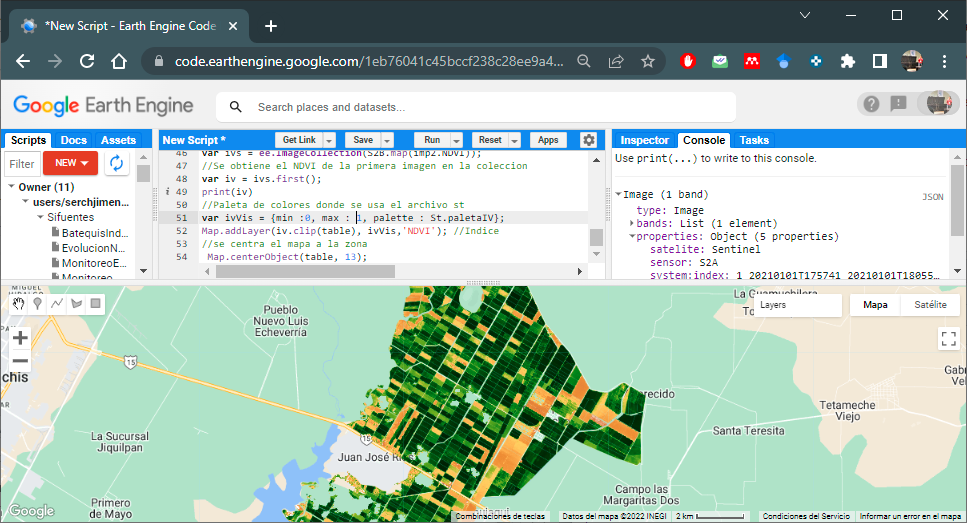
\includegraphics[width=0.85\linewidth]{./images/Figure74} 

}

\caption{mapa de NDVI para el area de interes}\label{fig:figV6}
\end{figure}

Para revisar el codigo del ejemplo clic \href{https://code.earthengine.google.com/299b022150c4569d006b323931f8d828}{aquí}

Si se desea visualizar el NDVI de una imagen en particular se debe convertir a lista de después mandar a llamarlo.

\begin{table}

\caption{\label{tab:Index}Codigo de indices de vegetación considerados en VICAL}
\centering
\begin{tabular}[t]{lcccc}
\toprule
Numero & Indice & Abreviatura & ExpresionGEE & Coeficientes\\
\midrule
1 & Atmospherically resistant vegetation index & ARVI* & ARVI & γ=1.0\\
2 & Adjusted transformed soil-adjusted vegetation index & ATSAVI* & ATSAVI & \\
3 & Difference vegetation index & DVI & DVI & \\
4 & Enhanced vegetation index & EVI & EVI & C1=6.0, C2= 7.5; L=1.0\\
5 & Enhanced vegetation index & EVI2* & EVI2 & C1=2.4\\
\addlinespace
6 & Green normalized difference vegetation index & GNDVI & GNDVI & \\
7 & Modified soil adjusted vegetation index & MSAVI2 & MSAVI2 & \\
8 & Moisture stress index & MSI & MSI & \\
9 & Modified triangular vegetation index & MTVI & MTVI & \\
10 & Modified triangular vegetation index-2 & MTVI2 & MTVI2 & \\
\addlinespace
 &  &  &  & \\
11 & Normalized difference tillage index (NDTI) & NDTI & NDTI & \\
12 & Normalized difference vegetation index & NDVI & NDVI & \\
13 & Normalized difference water index & NDWI & NDWI & \\
14 & Optimized soil adjusted vegetation index & OSAVI* & OSAVI & X=0.16\\
\addlinespace
15 & Renormalized difference vegetation index & RDVI & RDVI & \\
16 & Redness index & RI & RI & \\
17 & Ratio vegetation index & RVI & RVI & \\
18 & Soil adjusted vegetation index & SAVI* & SAVI & L=0.5\\
19 & Triangular vegetation index & TVI & TVI & \\
\addlinespace
20 & Transformed soil adjusted vegetation index & TSAVI* & TSAVI & a= 1 ; b=0;\\
21 & Visible atmospherically resistant index & VARI & VARI & \\
22 & Vegetation index number or simple ratio & VIN & VIN & \\
23 & Wide dynamic range vegetation index & WDRVI* & WDRVI & α=0.2\\
\bottomrule
\end{tabular}
\end{table}

\hypertarget{citar}{%
\chapter{Citar}\label{citar}}

\hypertarget{actualizaciones}{%
\chapter{Actualizaciones}\label{actualizaciones}}

Si tiene preguntas o encuentra que las actualizaciones introducen errores, envíe un correo electrónico a Justin a: \href{mailto:jimenez.sergio@inifap.gob.mx}{\nolinkurl{jimenez.sergio@inifap.gob.mx}}

\hypertarget{de-mayo-del-2022}{%
\section{02 de Mayo del 2022}\label{de-mayo-del-2022}}

-El usuario puede ingresar la \textbf{URL} de un archivo vector cargado desde GEE.
-Se puede exportar el polígono digitalizado en formato \emph{.kml.}

  \bibliography{book.bib,packages.bib}

\end{document}
